%Chapter 5: Offshore Data and Tsunami Modeling

\chapter{Offshore Data and Tsunami Modeling}

The rapid estimation of realistic tsunami models along the coast immediately adjacent to large earthquakes (the �``near-field'' or ``near-source'' region) continues to be a pressing problem for tsunami warning, as the number of people and infrastructure located in areas of tsunami hazard grows \citep{basher2006}. Tsunamigenic earthquakes in the last decade have had catastrophic consequences with a large loss of life and impact on the built and natural environments. Most notably the 2004 Mw 9.2 Sumatra-Andaman event \citep{ammon2005,ishii2005,lay2005,stein2005,subarya2006} resulted in over 250,000 casualties, the majority of them on the nearby Sumatra mainland, with run-up heights of up to 30m \citep{paris2007}. The Mw 8.8 2010 Maule earthquake in Chile \citep{lay2010,delouis2010} resulted in 124 tsunami related fatalities and run-up heights as high as 15-30m in the near-source coast \citep{fritz2011}. The 2011 Mw 9.0 Tohoku-oki earthquake \citep{simons2011,lay2011japan} generated a tsunami with inundation amplitudes as high as 40m  resulting in over 15,000 casualties \citep{mori2012} and was the first case of a large tsunami impinging upon a heavily developed and industrialized coastline in modern times. Tsunami induced damage was heavy on port infrastructure, major roadways and railways were severed, energy generating power stations (in particular, nuclear power) were forced offline for extended periods of time, defense infrastructure was compromised, and telecommunications were impeded as well as destruction of countless homes, offices and other industries. In addition to the tragic loss of life the economic collapse of the near-source coastline, which spans nearly 400km, was almost complete \citep{hayashi2012}. Throughout this chapter we will focus on how the techniques developed in Chapters 3 and 4 to rapidly image the earthquake source can be utilized to forecast tsunami intensity. Furthermore, we will demonstrate that land-based sensors alone provide only limited forecasts and that utilizing ocean-based measurements int he source estimation process greatly improves estimates of the earthquake source as well as tsunami forecasting and modeling.

\section{Background}

Japan possesses the only fully operational tsunami early warning system (TEW) worldwide capable of delivering alerts in the near-source coastline as well as numerous defenses against tsunami attack such as seawalls. The Tohoku-oki event demonstrated that early warning must be complemented with a comprehensive understanding of regional hazards and a prepared response in order to have the greatest impact. It also underscored some significant limitations of existing TEW methods, particularly in the near-field. Currently, operating algorithms to rapidly estimate tsunami intensity can be broadly divided into two classes: (i) those that use rapid estimates of simple earthquake source parameters like epicenter and magnitude, derived from land-based sensors, to guide warning and (ii) those that use direct measurements of sea-surface disturbances from ocean-based sensors to assess the intensity of an event without the need to characterize the earthquake source. The system of the Japanese Meteorological Authority (JMA) \citep{tatehata1997} is of the first kind; rapid determination of magnitude and event location from seismological measurements is used to seed a database query of pre-computed scenarios. These scenarios, determined well in advance of an event, are earthquakes of different magnitudes and locations that are used offline as initial conditions to produce simulations of tsunami propagation and metrics of inundation intensity at points along the Japanese coastline. Thus, when an earthquake strikes, from its rapidly determined magnitude and location the most appropriate scenario is extracted from the database and used to guide the warning. 


During the Tohoku-oki earthquake, early estimates of earthquake magnitude from JMA were too low by 1-2 orders of magnitude; an estimate of Mw 7.2 was determined after 30s and revised to Mw 8.0 by 107s \citep{hoshiba2011}. It took 20 minutes for a reliable estimate of magnitude to be made teleseismically through the W phase method \citep{duputel2011,hayes2011}. Maximum tsunami amplitudes of $\sim$40 m \citep{mori2012} were reached in the Sanriku coast within 30 minutes of rupture initiation. The underestimate of the earthquake size lead to early estimates of wave heights that were too low by several meters to tens of meters \citep{ozaki2011}. These complications in adequate magnitude estimation arise from reliance solely on seismic data to compute source parameters. Weak-motion seismometers, traditionally used for such tasks as monitoring local seismicity or Earth structure studies with teleseismic data, mechanically clip during strong shaking. Strong-motion accelerometers, designed to stay on-scale during periods of intense shaking, but, as demonstrated throughout Chapter 2, are not easily integrated to displacement because of unresolved baseline offsets in the acceleration data \citep{Boore2005}. Numerous schemes have been proposed to correct strong motion data and deal with this difficulty and a few of them show encouraging results and could possibly be automated \citep{Wang2013}. However even when strong motion waveforms are corrected carefully, it remains exceedingly hard to ensure that a corrected record reflects ground motion across the frequency band necessary to adequately characterize large sources. In Chapters 3 and 4 we showed that the long-period band of a record is the most critical to accurate magnitude computation of large events. Yet, in real-time inertial strong motion sensors it remains the most unreliable one, leading to saturation of near-source magnitude computations which result in underestimation of the earthquake size.


The second form of warning relies on direct measurements of sea-surface height disturbances ($\eta$). Most notably used for this purpose are the Deep-ocean Assessment and Reporting of Tsunamis (DART) buoys. They compose a network of ocean bottom pressure sensors installed in deep water (4000-6000m), acoustically relaying pressure information to a buoy equipped with satellite telemetry that communicates with a centralized processing facility \citep{gonzalez2005,mungov2013}. One reason for deploying in deep water is that the propagation of tsunami waves can be considered a linear process while in shallower water the non-linear behavior increases \citep{arcas2012} complicating the analysis of the tsunami source and forecasting. With these deep water measurements a linear inverse problem is solved for the tsunami source by superposition of previously computed unit sources of vertical seafloor displacement. This tsunami source is then used as the initial conditions in propagation of tsunami waves on a nested grid by solving the shallow water equations with numerical dispersion to simulate physical dispersion \citep{titov1997}. Once tsunami propagation has been modeled it is analyzed to generate site-specific warnings \citep{titov2005}. This approach has the advantage that it directly measures the tsunami rather than just rely on estimates of the size of the seismic source. However, bottom-pressure recordings like DART are expensive and sparse and because they are not deployed in the near-source coast provide no warning in the region immediately adjacent to the event. This method of warning has been mostly employed for ocean basin-wide forecasts.


With advances in real-time GPS such as instantaneous relative positioning \citep{bock2000,Bock2004,Larson2003} and precise point positioning \citep{Zumberge1997}, after the 2004 Sumatra event proposals for tsunami warning based on geodetic measurements and earthquake source models more complex than just magnitude and location emerged in the literature. \citep{Blewitt2006} used permanent deformation estimates produced by the earthquake from GPS to grid search a database of possible, pre-computed, earthquake finite fault models. \citep{sobolev2007}proposed and demonstrated the viability of a system that uses coseismic offsets from GPS to directly invert for a heterogeneous slip model. In the intervening period, before the 2011 Tohoku-oki event, the W phase method for computation of centroid moment tensors \citep{kanamori2008} started producing rapid solutions with far-field seismic data routinely \citep{hayes2009}. The  \textit{fast}CMT algorithm discussed in Chapter 3 also demonstrated that CMTs could be computed with coseismic offsets from GPS, without regard for saturation at high magnitudes, a problem often faced by seismic methods. \citep{otoole2012} demonstrated the viability of full waveform CMT inversions from the high-rate real-time GPS data. \citep{singh2012} tested an algorithm for estimation of rapid rectangular source models with uniform slip and \citep{Crowell2012} produced heterogeneous coseismic slip inversions from real-time data for two large events. The pace of research in the field accelerated after the 2011 Tohoku-oki event. \citep{guilhem2013} as well as our own work that extends the \textit{fast}CMT algorithm to a line source are a solution to the problem of violation to the point source assumption often faced with near-field CMT determination of large events. \citep{Ohta2012} were able to produce in simulated real-time mode a simple uniform slip source model for the 2011 Tohoku-oki event; \citep{PerezCampos2013} computed similar models for one scenario and one recorded subduction event in Mexico. \citep{Wright2012} produced source models with 4 fault patches from precise point positioning data. 


Furthermore, we've shown in Chapter 3 that a slip inversion, in simulated real-time mode, for the Tohoku-oki event from improved coseismic offsets by the optimal combination of accelerometer and GPS data is possible. This was achieved through a Kalman filter formulation (Chapter 2). Notably, in Chapter 3 we've shown that the fault plane used for the slip inversion can be determined without operator interaction, a problem not addressed before, by means of a finite-extent line source CMT inversion that bounds the geographic extent of moment release. This is important because a CMT determination allows discernment between thrust, normal and strike-slip events, all of which are possible in a subduction setting, but pose distinct tsunami hazards. This often ignored step is crucial because not all large events in a subduction zone can be assumed to happen on the megathrust. The Mw 8.6 event off Sumatra, Indonesia, on 11 April 2012 \citep{satriano2012} was a predominantly strike-slip event that produced no significant tsunami. Similarly, the Mw 8.1 Samoa event on 29 September 2009 was a normal faulting, outer-rise type event that produced a sizable tsunami with 189 fatalities \citep{okal2010}. More recently the 2012 Mw 7.8 Haida Gwai thrust event offshore British Columbia produced a tsunami and was followed 2 months later by a Mw 7.5 strike-slip event on the fore-arc sliver \citep{lay2013}. Additionally the availability of a finite-extent CMT estimate is crucial to determining the fault plane on which to parameterize the slip inversion. We've argued throughout this work that geodetic and especially seismogeodetic data can rapidly characterize earthquakes of arbitrarily large magnitude and faulting type with minimum assumptions.


This extensive body of research by the community cohesively argues that improved earthquake source models should play an important role in guiding tsunami warning. However, in spite of mentioning that source characterization could aid tsunami warning, before \citet{Ohta2012}, none of the above works gauged the impact of their source models on inundation forecasting. Neither did they propose how to map an earthquake source estimate into a forecast of tsunami intensity. This class of warning, where a tsunami propagation model is initiated from an earthquake source inversion, is often called indirect \citep{arcas2012} because it does not involve measurement of the tsunami itself. \citet{Ohta2012} used their uniform slip source estimates as initial conditions for a tsunami that they propagated using the algorithm of \citet{tsushima2009}, which assumes tsunami Green functions (tGF) from unit sources of vertical sea floor displacement \citep{satake1995}, and compared it with off-shore GPS buoys, bottom pressure sensors and tide gauges with mixed results.


\citet{macinnes2013} tested ten source models obtained from inversion of GPS, far-field seismic and tsunami wave gauge data as initial conditions to model tsunami propagation. When simulation results were compared to DART buoys and post-event field survey measurements \citep{mori2012}, it was found that indeed the diversity of source models produces significant variations in the simulated tsunami. This reiterates a recurring problem in tsunami science; for indirect warning the non-uniqueness of source inversions poses a hurdle. However \citet{macinnes2013} showed that in spite of this, many source models retain the capacity to produce realistic tsunami scenarios. The source inversion techniques analyzed in that study, however, are problematic for real-time implementation. They rely heavily on far-field geophysical data as well as decision-making by the researcher to define the parameterization to be used in the inverse problem. \citet{hoechner2013} also produced tsunami intensity estimates in the near-source coastline from a 30 s sampled GPS-derived static slip inversion; that work however did not asses the accuracy of the inundation model or provide an automated way to determine faulting style, select the slab segment or determine the regularization parameter in the inverse problem.


Additionally, offshore shallow water measurements from coastal tide gauges, GPS buoys and ocean bottom pressure sensors can be used in a linear inverse problem \citep{satake2013} for the earthquake source. Furthermore the joint inversion of both data sets \citep{romano2012,gusman2012} produces a slip pattern significantly different from the land-based static offset inversions only of \citet{hoechner2013} and Chapter 3, albeit with similar seismic moment. This is important because it suggests that indirect warning can then rely on actual measurements of tsunami propagation to improve the earthquake source model.


Follwing we will demonstrate first the improv,nets from static-offset derived models since these are the ones easiest to compute and that necessitate the fewest assumptions. We will employ line-source CMT and finite fault slip models derived from a seismogeodetic analysis of Chapter 3 and tsunami wave gauge data for the 2011 Tohoku-oki event to accurately forecast the tsunami intensity and inundation levels. We will emphasize the need for careful algorithm design to ensure minimal interaction from the network operator and assure that the process can be fully automated. This multi-sensor approach can then be applied as a basis for more timely and effective early warning for residents of the near-source coastline.


\section{Static Modeling: Data and Method}

\label{sec:method}

\subsection{Description}

The real-time combination of strong motion and GPS data via a multi-rate Kalman filter produces broadband strong motion displacement waveforms (Chapter 2) that are reliable at all frequencies of seismological interest. These seismogeodetic data, can be used in a real-time environment to obtain high accuracy coseismic offsets and rapidly compute line-source CMT solutions and finite fault slip models as a regularized linear inverse problem (Chapter 3). We use  the same data as before, from 139 collocated GPS and accelerometer station pairs (within 1.5 km) in Japan (Figure \ref{fig_maps}) in the computations for the 2011 Mw 9.0 Tohoku-oki earthquake. A finite extent CMT solution is calculated with the fastCMT algorithm to determine type of faulting and geographical extent of rupture, followed by estimation of a finite fault slip model. The regional 3D slab model for the subduction zone is established a priori from \citet{hayes2012}. In a real-time scenario, the relevant segment of the slab is extracted from the regional model based on the moment release of the finite extent CMT. It is then discretized to sub-fault patches and the slip inversion is performed. This approach using the seismogeodetic data yields slip inversions with more shallow slip than the GPS-only inversions due to improved precision in the vertical channel. This distinction is critical, while the algorithm described here can be employed with GPS data alone, the addition of the strong motion data reduces the uncertainty of the vertical component of motion. For the Tohoku-oki case this model is determined at 157s after earthquake origin time and in the timeline of warnings provides the first estimate of the slip distribution.

\begin{figure}[!ht] 
  \centering
  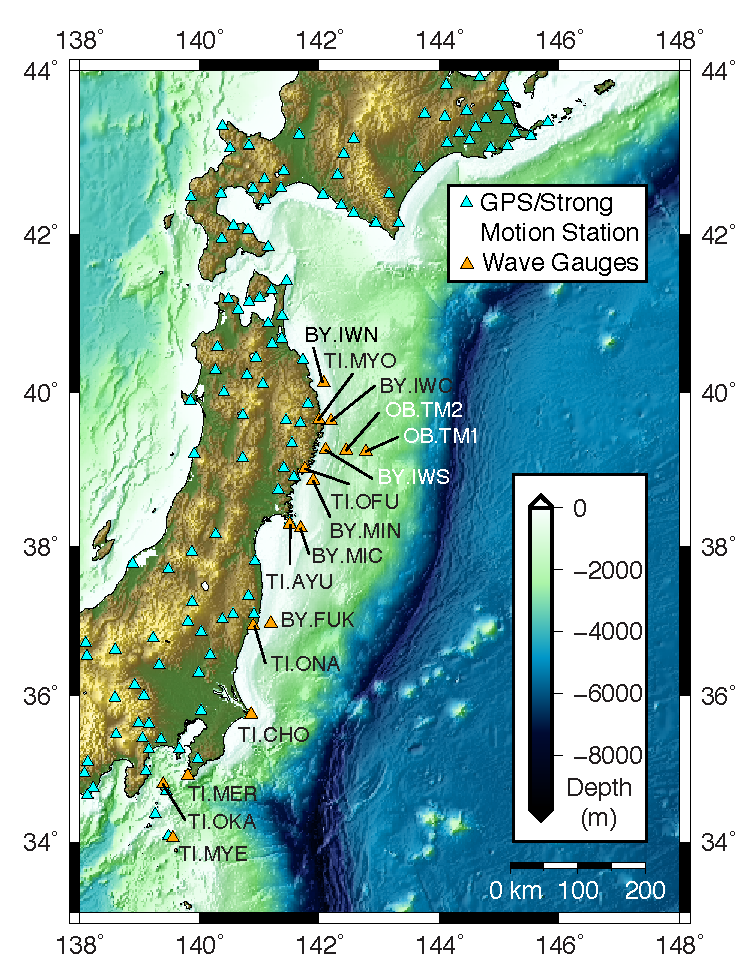
\includegraphics[width=0.75\linewidth]{./figures/ch5/map.pdf}
    \caption[Tohoku-oki station map]{Distribution of stations used in this study. Blue triangles are land-based GPS/strong motion stations. Orange triangles are ocean-based stations: tide gauges (labeled TI), GPS Buoys (labeled BY) and cabled ocean bottom pressure sensors (labeled OB).}
  \label{fig_maps}
\end{figure}

As time progresses data from coastal and offshore wave gauges begin to accrue and are incrementally ingested into the inversion process. We employ data from 8 coastal tide gauges, 6 off-shore GPS buoys and 2 ocean bottom pressure (OPB) sensors for a total of 16 wave gauges (Table \ref{tb_wave_stations}, Figure \ref{fig_maps}). The data for all stations are resampled at 15 s. To compute the tGFs we calculate the seafloor deformation for 1 m of thrust and 1 m of strike-slip motion at each one of the subfaults. We then compute the resulting tsunami waveform at each one of the 16 wave gauges from this unit amount of slip using the open source GeoClaw software (www.clawpack.org). These time series of sea-surface motion are what we consider the tsunami Green functions for every subfault wave gauge pair.

\begin{table}
\caption[Stations used in the inversion]{Wave gauges used in the inversion. All the time series are resampled to 15 s. The agencies responsible for the stations are the Earthquake Research Institute (ERI), the Nationwide Ocean Wave information network (NOW) and the Japan Meteorological Agency (JMA).}
\label{tb_wave_stations}
\begin{tabular}{l l l r r r r}
\hline
Station & Instrument & Code & Lat ($^\circ$) & Lon ($^\circ$) & Depth\\
\hline
TM1	& OBP & OB.TM1 & 142.7683 & 39.2311	& 1618\\
TM2 & OBP & OB.TM2 & 142.4411 & 39.2489 & 1013\\
Fukushima & GPS Buoy & BY.FUK & 141.1856	 & 36.9714 & 137\\
Central Iwate & GPS Buoy & BY.IWC & 142.1867 & 39.6272 & 200\\
Northern Iwate & GPS Buoy & BY.IWN & 142.0667 & 40.1167 & 125\\
Southern Iwate	& GPS Buoy & BY.IWS & 142.0969 & 39.2586 & 204\\
Central Miyagi	& GPS Buoy & BY.MIC & 141.6836 & 38.2325 & 144\\
Northern Miyagi & GPS Buoy & BY.MIN & 141.8944 & 38.8578 & 160\\
Ayukawa & Tide Gauge & TI.AYU  & 141.5002  & 38.2820 & 0\\
Choshigyoko & Tide Gauge & TI.CHO & 140.8583 & 35.7444 & 0\\
Mera	 & Tide Gauge & TI.MER & 139.8023 & 34.9056 & 0\\
Miyakejima Tsubota & Tide Gauge & TI.MYE & 139.5518 & 34.0459 & 0\\
Miyako & Tide Gauge & TI.MYO & 141.9864  & 39.6396 & 0\\
Ofunato & Tide Gauge & TI.OFU & 141.7529  & 39.0066 & 0\\
Okada & Tide Gauge & TI.OKA & 139.3913  & 34.7894 & 0\\
Onahama & Tide Gauge & TI.ONA & 140.8919 & 36.9369 & 0\\
\hline
\end{tabular}
\end{table}

We ingest the tsunami observation data in 10 minute increments and jointly invert them with the seismogeodetic offsets assigning relative weights of 1 to the tide gauges, 5 to the GPS-buoys and 10 to the ocean bottom pressure sensors \citep{satake2013}. These weights arise from an analysis in Section \ref{sec:linearity} on the linearity of tsunami propagation at the different sensor locations. They are also in line with recent inversion techniques that employ these data \citep{satake2013}. We thus have a source estimate at 157s after rupture initiation from just the seismogeodetic data  and then at 10, 20, 30, 40 and 50 minutes from the joint inversion of land- and ocean-based data for a total of 6 models. The segment of the slab where the inversion is performed is that determined from the line source CMT in Chapters 3 and 4 and is held fixed throughout. For automated selection of smoothing in the slip inversions we, once again, employ Akaike�s Bayesian Information Criterion. At each instance we compute 200 slip inversions with varying degree of smoothing and select as our preferred model the one with smallest ABIC. The computation of 200 source models takes only a few minutes on a four-core computer and is easily parallelizable since each computation is independent of the others.

For each preferred source model (the one with smallest ABIC) we compute the predicted vertical seafloor deformation and use it as the initial condition for a tsunami simulation. To propagate the tsunami we employ GeoClaw (http://clawpack.org), by which two-dimensional shallow water equations are solved with the finite volume technique \citep{leveque2002}. The code simulates non-linear water wave propagation and can deal with discontinuities in the solution, such as turbulent bore formation, by shock capturing. Furthermore it employs adaptive mesh refinement (AMR) such that regions of larger tsunami complexity are automatically refined to higher discretization levels according to heuristics prescribed by the user. The code is suitable for near shore inundation analysis. It employs a Manning-type law for bottom friction (we held the coefficient fixed at 0.025) and has a moving sea/land boundary condition that allows cells to be wetted or dried as the simulation progresses and has a non-reflecting outflow boundary condition at the edges of the model domain. The algorithms are described in detail in \citet{george2006}, \citet{george2008} and \citet{berger2011}. GeoClaw has been benchmarked by the National Tsunami Hazard Mitigation Program (NTHMP) \citep{gonzalez2011} and approved for use in hazard modeling products. A simulation run takes $\sim$1 hour on the same four-core computer using the standard open source multi-processor platform openMP. Ostensibly for real-time performance the code can be optimized and the run time can be significantly improved by parallelization to a suitable level.

Topography for the simulations is taken from the Shuttle Radar Topography Mission (SRTM3) \citep{farr2007} with a resolution of 3 arcseconds ($\sim$90m pixel size). Off shore bathymetry has a resolution of 30 arcseconds ($\sim$1km pixel size) from the SRTM30+ dataset \citep{becker2009,sandwell2009}, which represents a synthesis of marine soundings and spaceborne altimeter measurements. The vertical datum of both data sets is mean seal level (MSL).

The simulations are run for 120 minutes of model time with output at 15s intervals. The simulation domain is between 34$^\circ$N and 41$^\circ$N and 139$^\circ$E and 146$^\circ$E. From the model output we extract 2 distinct sets of inundation information. First, we collect maximum inundation amplitudes at the coordinates of 2256 quality A and B survey measurements located inside the model domain from \citet{mori2012}. We also collect the inundation amplitude at all points on the coastline (at mean sea level, MSL) as defined by the SRTM3 water body data information. For each point where inundation output is desired we use the finite volume cell whose center is nearest the observation point at any given instant. The distinction between these two types of inundations can be appreciated in Figure \ref{fig_cartoon}. Inundation at the coastline is the maximum amplitude of the tsunami at the water-land boundary as defined before the event and it is equal to the maximum flow depth at that point. The inundation at the survey points is the maximum amplitude of the flow, with respect to the vertical datum defined by MSL. It�s inundation at a point that is on land before the event. The inundation amplitudes at the survey points are not the amplitude of the tsunami with regards to the local elevation (the flow depth). The inundation at the survey points is used to verify the predictive power (often referred to in forecasting as the skill of the model) of each simulation. In contrast the predicted inundations at the coastline are what we propose could be used as intensity metric to guide the warning. The simulations also produce wave gauge output at the locations (Figure \ref{fig_maps}) of the ocean bottom pressure sensors, GPS buoys, and tide gauges located along the coast.

\begin{figure}[!ht] 
  \centering
  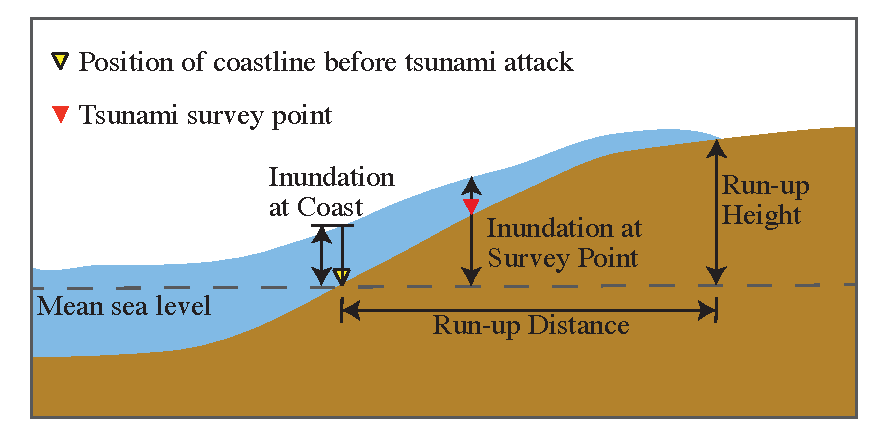
\includegraphics[width=0.9\linewidth]{./figures/ch5/inund_cartoon.pdf}
    \caption[Definition of tsunami inundation]{A schematic of the measures of tsunami intensity used in this study. The inundation at the coast and the inundation at the survey points from \citet{mori2012} are both referenced to the vertical datum defined by mean sea level.}
  \label{fig_cartoon}
\end{figure}

\subsection{Linearity in Tsunami Propagation}

\label{sec:linearity}

Underlying the joint inversion procedure is the assumption that tsunami propagation in shallow water (at the locations of the wave gauges) is a linear process. That is, tsunami waves generated by uplift due to slip on distinct subfaults can be linearly superimposed. Recent studies have made this assumption when using these measurements to analyze the earthquake source even at coastal tide gauges \citep{romano2012,gusman2012,satake2013} and indeed the same assumption is made in this study. However, it is well known that the non-linearity of tsunami propagation increases as the wave shoals. That linearity can be invoked for modeling with data from such shallow depths is controversial \citep{arcas2012} and the assumption that it cannot is one of the reasons for deploying DART buoys in deep water \citep{titov2005}. The GeoClaw simulation code solves the non-linear shallow water equations so it is possible to test this assumption, at least numerically, and at the level of precision allowed by the bathymetry and topography we employ here. 

We develop two simple tests of linearity. First we test for homogeneity to ensure that, for a given model, $f(x)$, $f(\alpha x)=\alpha f(x)$ where $\alpha$ is a scalar. We place 1m of thrust slip on a shallow fault patch in the middle of the fault model (patch 10) and simulate the tsunami, we then place 2m of slip on the same patch, simulate the tsunami and compare this output to the result of multiplying the output of the 1 m simulation by 2. The results are in (Figure \ref{fig_linearity1}). The second test is for additivity such that, for two models $f(x)$ and $f(y)$, $f(x+y)=f(x)+f(y)$. We again place 1m of slip on subfault patch 10 and place 1m of slip on a deeper subfault (patch 37). We model the tsunami from simultaneous slip on both patches and compare it to the addition of the output from the independent simulations of each fault patch (Figure \ref{fig_linearity2}). The results of these two tests show that non-linearities exist but that they are small compared to the maximum amplitude of the tsunami at each wave gauge. Also the non-linearities are larger at the tide gauges (which are in shallower water) than at the GPS buoys and OBP sensors. This is the reason for the relative weighting scheme discussed in the previous section. Generally the non-linearities are more pronounced at longer times after the first arrival. We perform similar analysis on different combinations of subfaults with similar results. We conclude that non-linearities exist, are quantifiable but small enough to allow for a joint inversion. Because non-linearities are smallest during the first wavelength of the tsunami the linearity assumption will degrade as longer and longer segments of the wave gauge record are used.

\begin{figure}[!ht] 
  \centering
  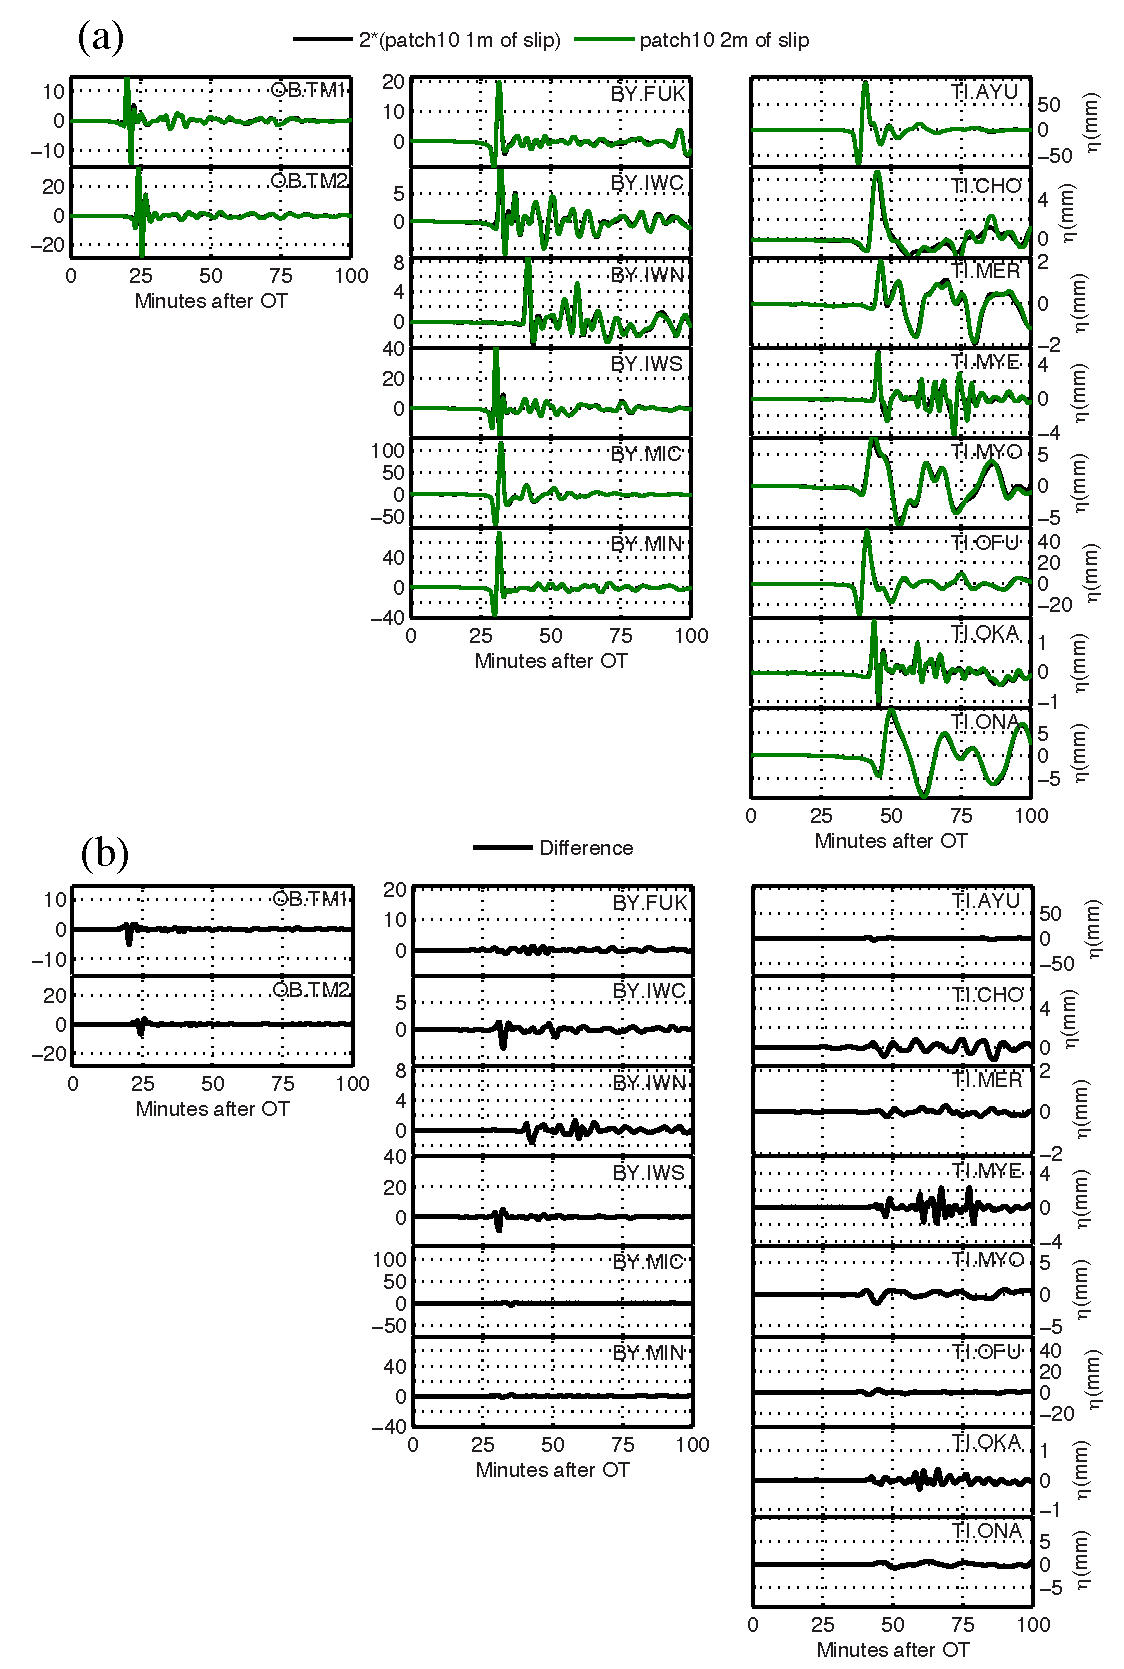
\includegraphics[width=0.8\linewidth]{./figures/ch5/linearity1.pdf}
    \caption[Linearity test No.1]{Result of testing the assumption of linearity in tsunami propagation. (a) is the result of testing for homogeneity, the black line is the result of the linear superposition and the green the result of the GeoClaw non-linear simulation. (b) is the difference between the two results}
  \label{fig_linearity1}
\end{figure}

\begin{figure}[!ht] 
  \centering
  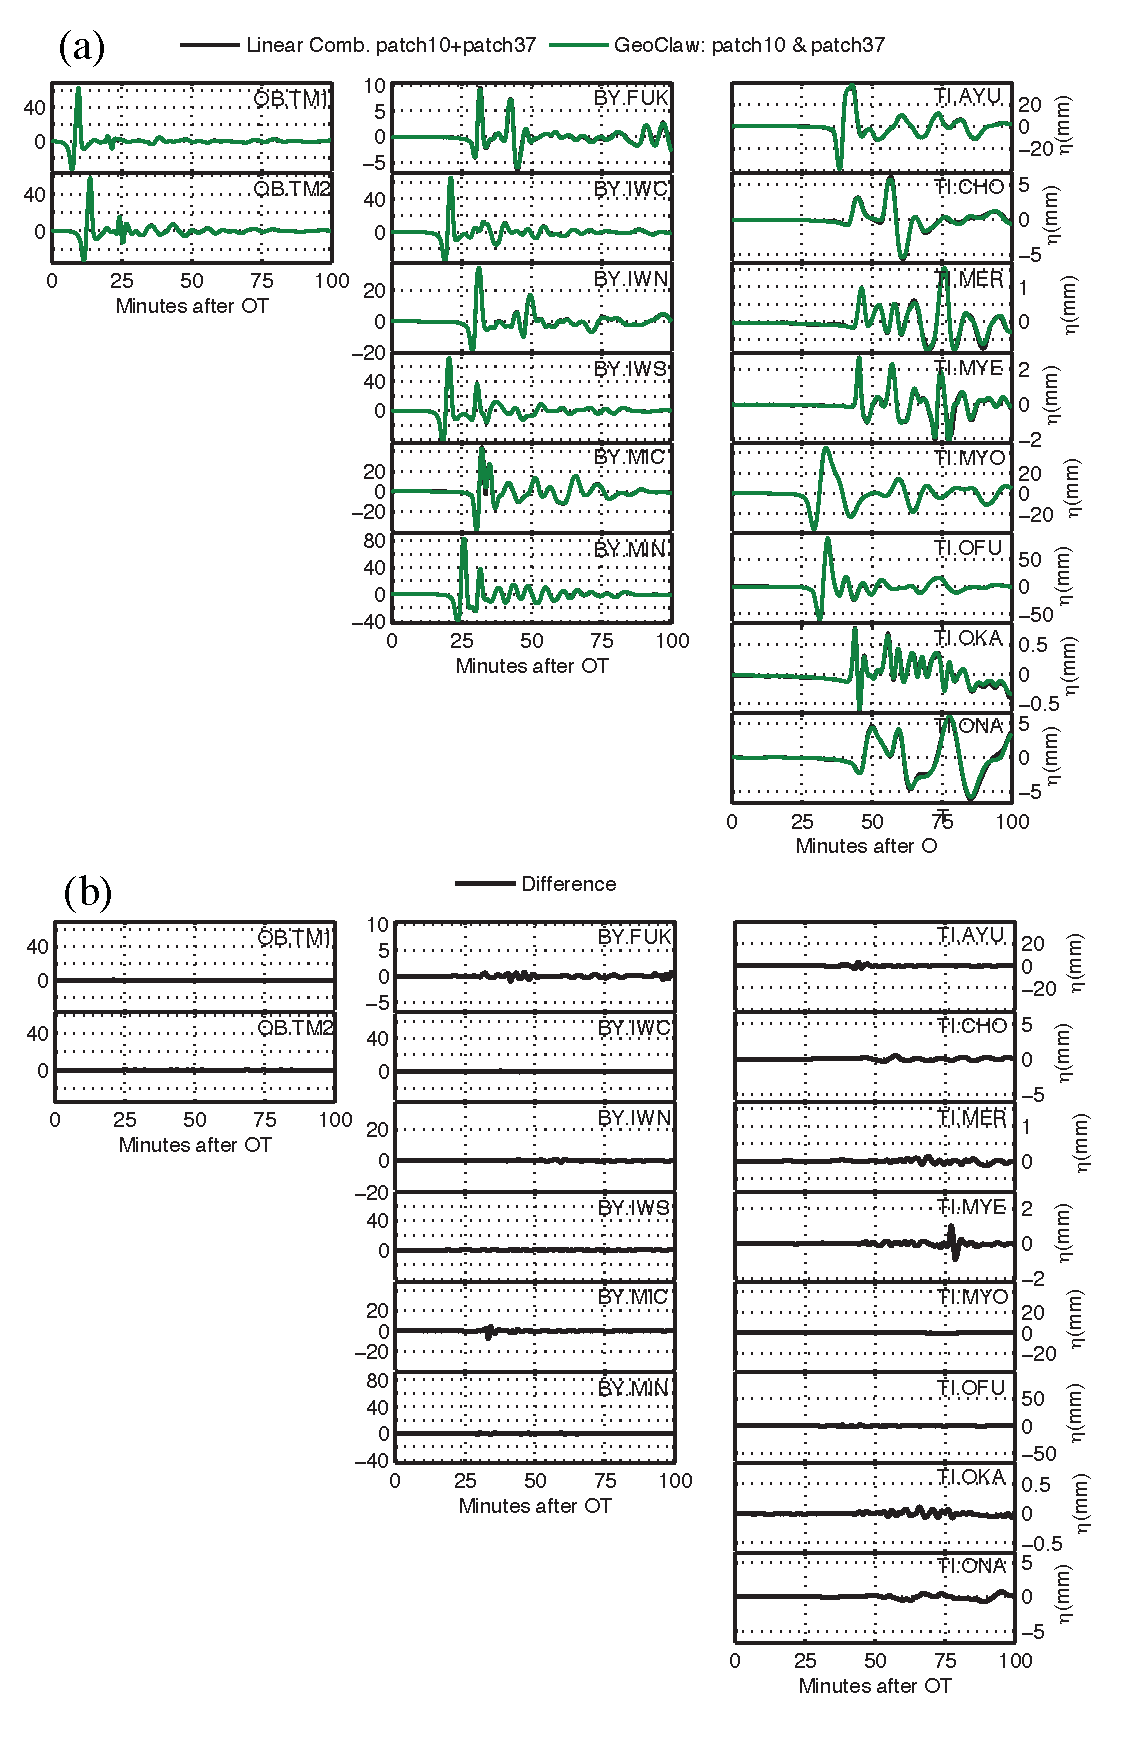
\includegraphics[width=0.8\linewidth]{./figures/ch5/linearity2.pdf}
    \caption[Linearity test No.2]{Result of testing the assumption of linearity in tsunami propagation. (a) is the result of testing for superposition, the black line is the result of the linear superposition and the green the result of the GeoClaw non-linear simulation. (b) is the difference between the two results}
  \label{fig_linearity2}
\end{figure}

\section{Inversion and Forecast Results}

The results of the inversions at the 6 time intervals are summarized in Figures \ref{fig_results1} and \ref{fig_results2} and Table \ref{tb_results}. Figure \ref{fig_results1} shows the results of the finite fault slip inversion from the land-based data obtained at 157s after earthquake origin time (OT). Peak slip as reported in Chapter 3 for the static case is close to 30m and maximum seafloor uplift is $\sim$6m. The fit to 50min of wave gauge data (Figure \ref{fig_results1}) (not used in the inversion) is poor, with a root mean square (RMS) value of 1.42m. The OBP stations are not well fit and the tsunami amplitude is underestimated; similar results are observed for the buoy measurements indicating that the tsunami is systematically underestimated. This rather smooth slip model, however, fits the coseismic offsets from the seismogeodetic data with a 99\% variance reduction (Table \ref{tb_results}). The joint inversion with the first 10 minutes (Figure \ref{fig_results1}) of wave gauge data shows minimal differences from the inversion using just the land data. The fit to the coseismic offsets is reduced slightly to 98\% variance reduction, and the fit to the 10 min of wave gauge data improves (RMS of 0.26 m). Only the pressure gauges have a significant signal of $\sim$1 m amplitude. The remaining stations have yet to register a significant disturbance. At 20 min (Figure \ref{fig_results1}) significant differences arise. The peak tsunami amplitude has been reached in the OBP records and all GPS buoys register a sizeable signal. As a result, the slip inversion is noticeably altered; it has a peak displacement of $\sim$60 m over a large asperity and peak seafloor uplift is $\sim$20 m. The fit to the wave gauge data is very good (RMS of 0.24m) while the fit to the coseismic offsets is significantly reduced to a variance reduction of 66\%. The magnitude has increased from Mw 8.9 in the previous inversions to 9.1. Between 30min and 50min (Figure \ref{fig_results2}) the inversion stabilizes as the first peaks of the tsunami waveform have been fit at the deeper water (TI and BY) stations (Table \ref{tb_wave_stations}); subsequent changes are a result of fitting the later part of the time series and the lower-weight coastal tide gauge data. Peak slip settles at around 60m on a very shallow patch at 38$^\circ$N and on a deeper patch at 15km depth around 37$^\circ$N; magnitude is Mw 8.98-9.04. The fit to the coseismic offsets over this period oscillates (Table \ref{tb_results}) and settles to 70\% on the last inversion while the fit to the wave gauges remains stable at ~0.9 m RMS. We note that the peak amplitudes at both pressure gauges and 4 of the 6 buoys are consistently well modeled. However, for two buoys, BY.IWC and BY.IWN off-shore Iwate prefecture, (Table \ref{tb_wave_stations}, Figure \ref{fig_maps}) the peak amplitude is underestimated by about 50\%. The tide gauges contribute little to the inversion since they receive the smallest weight and provide information too late to be of use for early warning for this event. We note that for two of the distant tide gauges, TI.CHO and TI.MYE, the peak amplitude is not well resolved (Figures \ref{fig_results1},\ref{fig_results2}). We also note that these two stations exhibit the strongest non-linear behavior (Figures \ref{fig_linearity1},\ref{fig_linearity2}). The tide gauge stations with small non-linear behavior and closest to the source (TI.AYU, TI.MYO and TI.OFU) appear to be well modeled, in spite of having a clipped record.

\begin{figure}[!ht] 
  \centering
  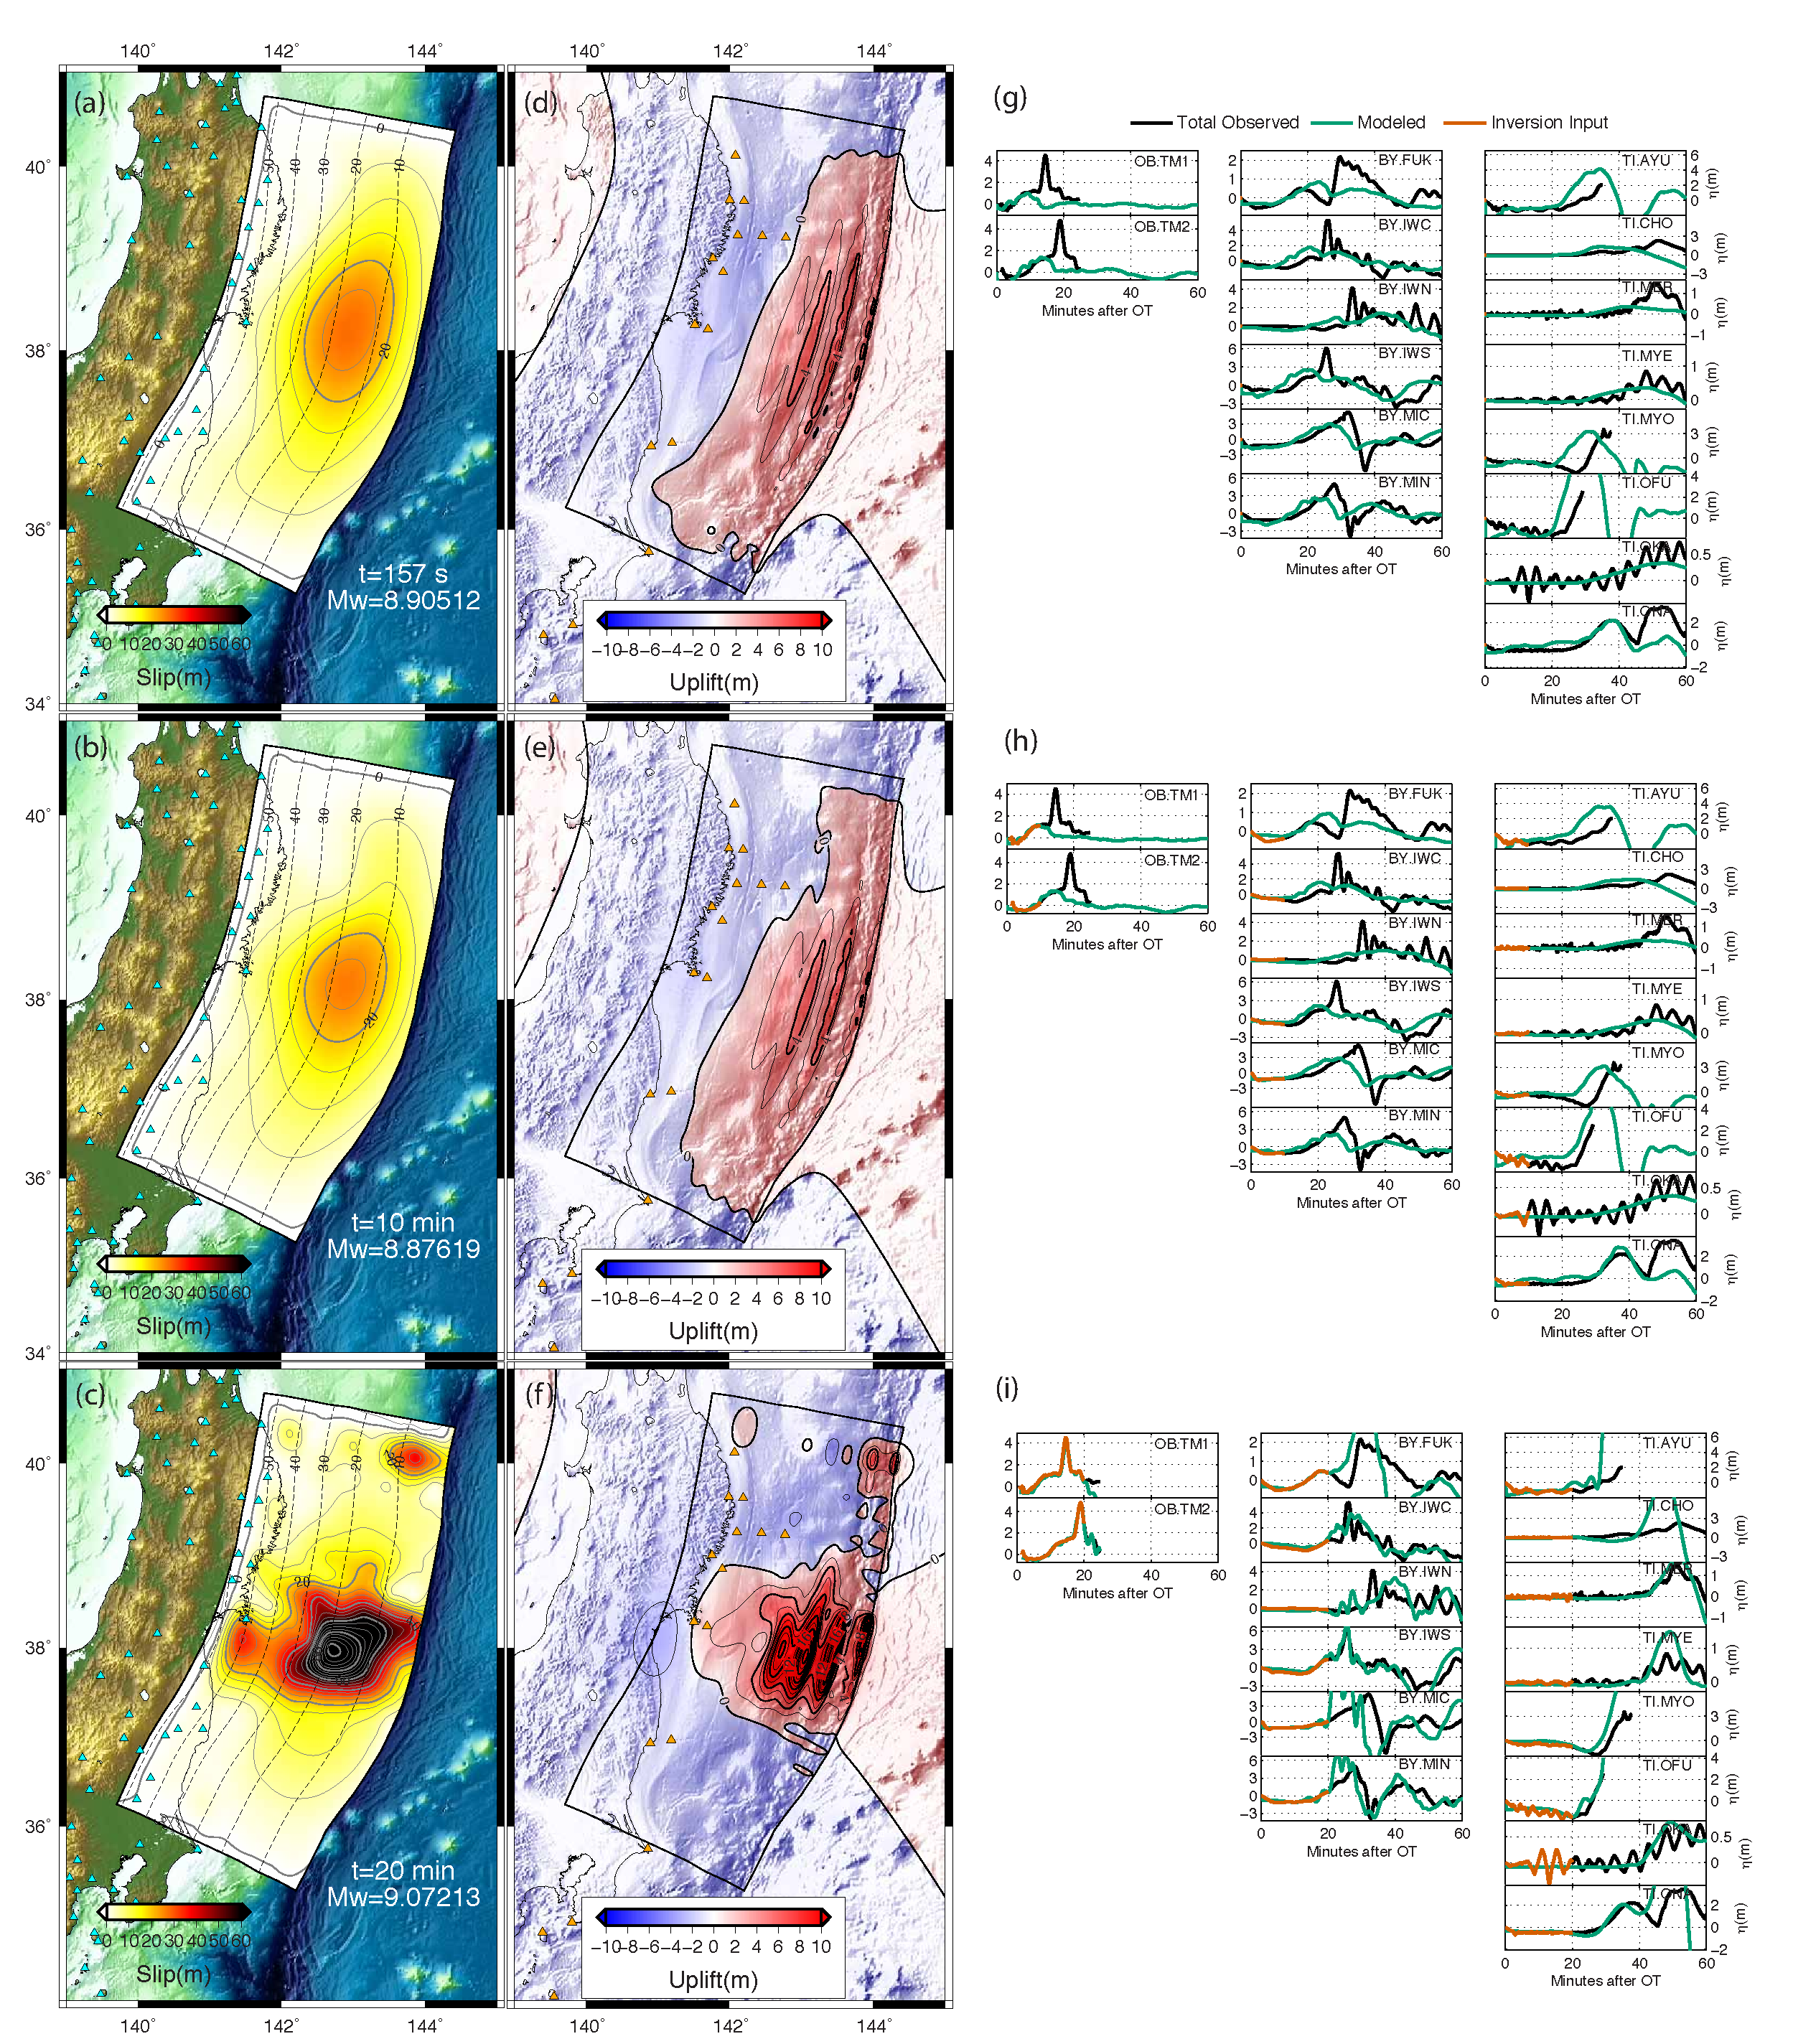
\includegraphics[width=0.99\linewidth]{./figures/ch5/results1.pdf}
    \caption[Inversion results No.1]{Inversion results. (a)-(c) Slip inversions at 157 s, 10 min and 20 min after earthquake origin time. The inversion at 157 s is from land-based measurements. Subsequent inversions are of the joint data set. Grey lines are the slip contours at 5 m intervals and black dashed lines are the slab depths. (d)-(f) Predicted seafloor uplift from the inversions. (g)-(i) Comparison between observed (black) and synthetic (green) data for the wave gauges. The orange portion of the waveforms is the input for the inversion.}
  \label{fig_results1}
\end{figure}

\begin{figure}[!ht] 
  \centering
  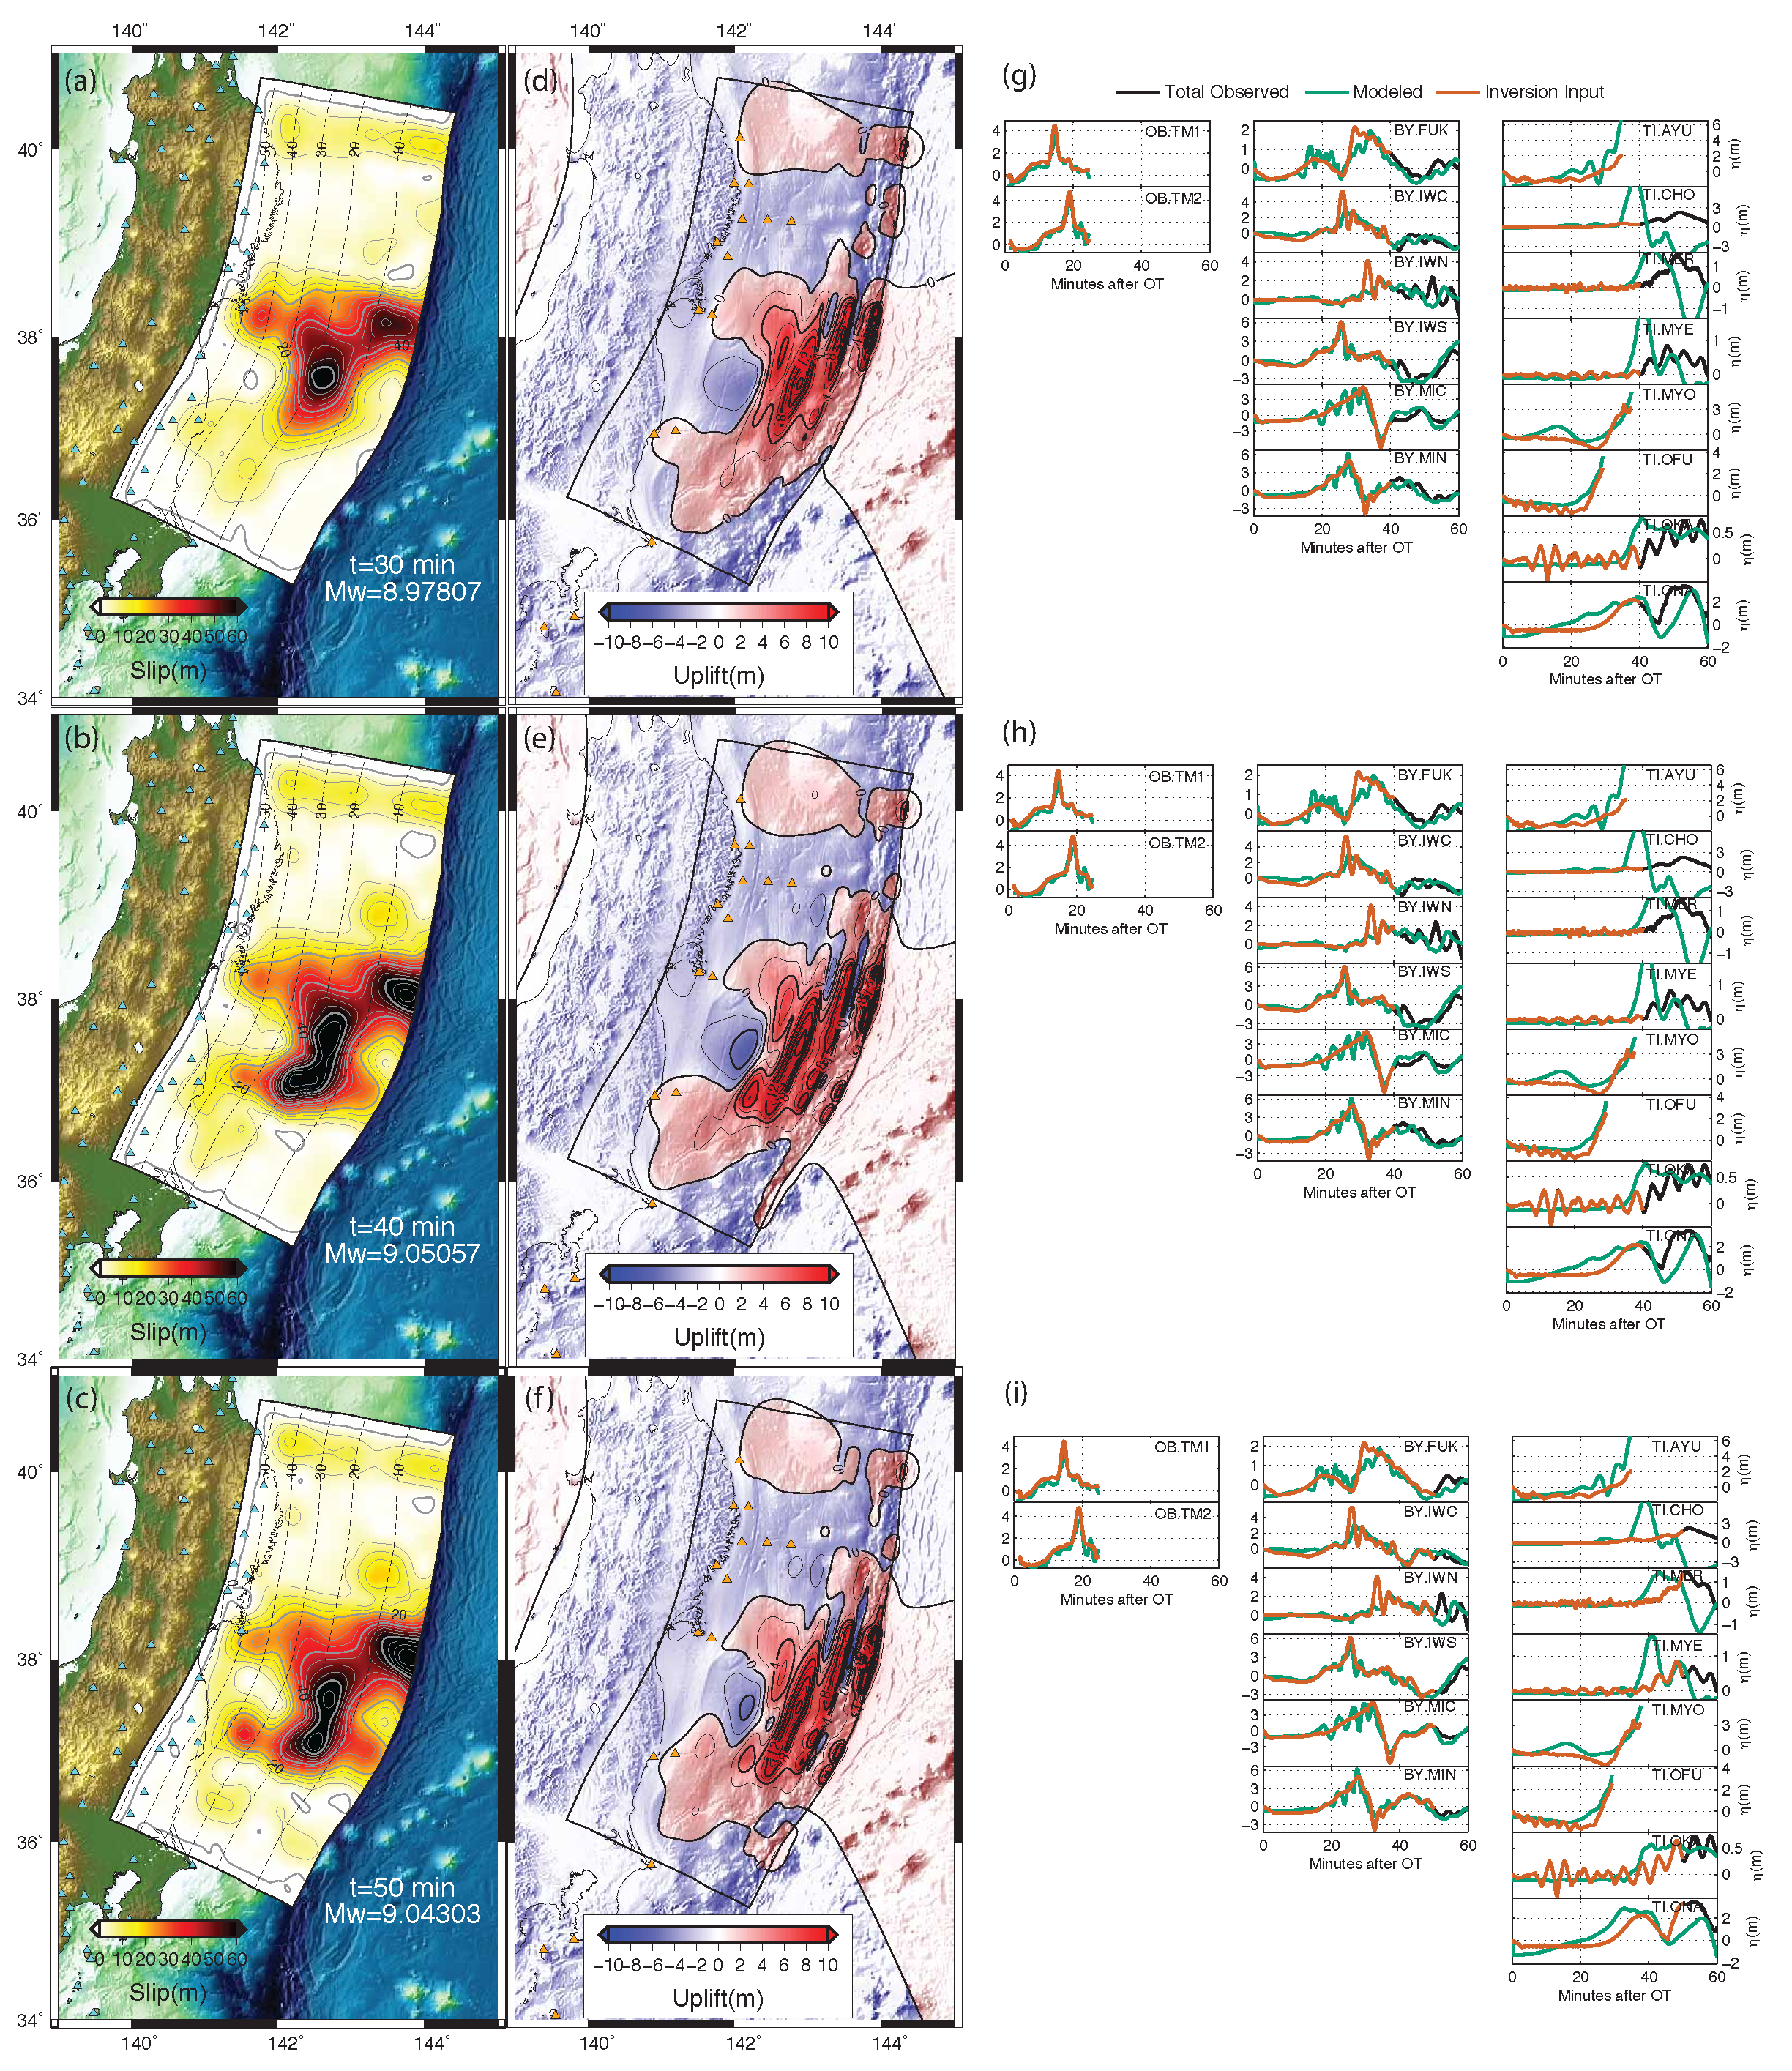
\includegraphics[width=0.99\linewidth]{./figures/ch5/results2.pdf}
    \caption[Inversion results No.2]{Inversion results. (a)-(c) Slip inversions at 30, 40 and 50 min after earthquake origin time. Inversions are of the joint data set. Grey lines are the slip contours at 5 m intervals and black dashed lines are the slab depths. (d)-(f) Predicted seafloor uplift from the inversions. (g)-(i) Comparison between observed (black) and synthetic (green) data for the wave gauges. The orange portion of the waveforms is the input for the inversion.}
  \label{fig_results2}
\end{figure}

\begin{table}
\caption[Inversion statistics]{Statistics of the inversions and inundation models. The first column is variance reduction (VR) between the coseismic offset measurements and the synthetic offsets from the inversion. The second column is RMS of the fit to the wave gauge measurements. The third column is variance reduction of the modeled inundation compared to the surveyed inundation from \citet{mori2012}. The 4th column is the number of inundation survey points inundated by the model}
\label{tb_results}
\begin{tabular}{l c c c c}
\hline
Time & Coseismic & Wave Gauge & Survey & Survey Points\\
 & VR(\%) & RMS (m) & VR(\%) & Inundated\\
\hline
157s	& 99 & 1.42 & 85 & 956/2250\\
10min & 98 & 0.26 & 79 & 905/2250\\
20min & 68 & 0.24 & 60 & 1913/2250\\
30min & 78 & 0.55 & 73 & 1538/2250\\
40min & 57 & 0.87 & 65 & 1604/2250\\
50min & 70 & 0.85 & 78 & 1611/2250\\
\hline
\end{tabular}
\end{table}


Using the slip inversions and seafloor uplift maps in Figures \ref{fig_results1} and \ref{fig_results2} we model the ensuing tsunami with GeoClaw as described in Section \ref{sec:method}. Figure \ref{fig_forecast} shows the maximum expected amplitude near the earthquake source. We note that the inversions at 157s and 10min that have little or no information from the wave gauges predict smaller amplitudes than the inversions relying on more complete wave gauge records. After 20 min a sizable tsunami is forecast in the near shore region. It is interesting to note a large lobe of high amplitude waves radiating in the trench normal direction. This lobe seems to initiate above the deeper (10-20 km) asperity in Figures \ref{fig_results1} and \ref{fig_results2} and not above the very shallow patch of high slip. At 50 minutes a second lobe of high amplitude is forecast to radiate from the very shallow patch of slip at 38$^\circ$N. The intersection of these high amplitude lobes with the coastline matches the pattern of maximum observed inundation amplitudes from the survey points (Figure \ref{fig_inundation}). For the smooth land-based models the first wave is almost continuous along the fault strike, however for the more complex models from the joint inversions the first pulse is broken into two or three distinct waves that jog along strike. There are persistent oscillations in Sendai bay and the smaller inlets of the Sanriku coast (38$^\circ$N to 40$^\circ$N) and along the continental shelf akin to basin and shelf resonance. Diffraction along the Oshika peninsula that juts north of Sendai bay is also apparent. The complex behavior in the models shows the repeated and long-lasting attack of multiple waves on the coastline after the main arrival. 

\begin{figure}[!ht] 
  \centering
  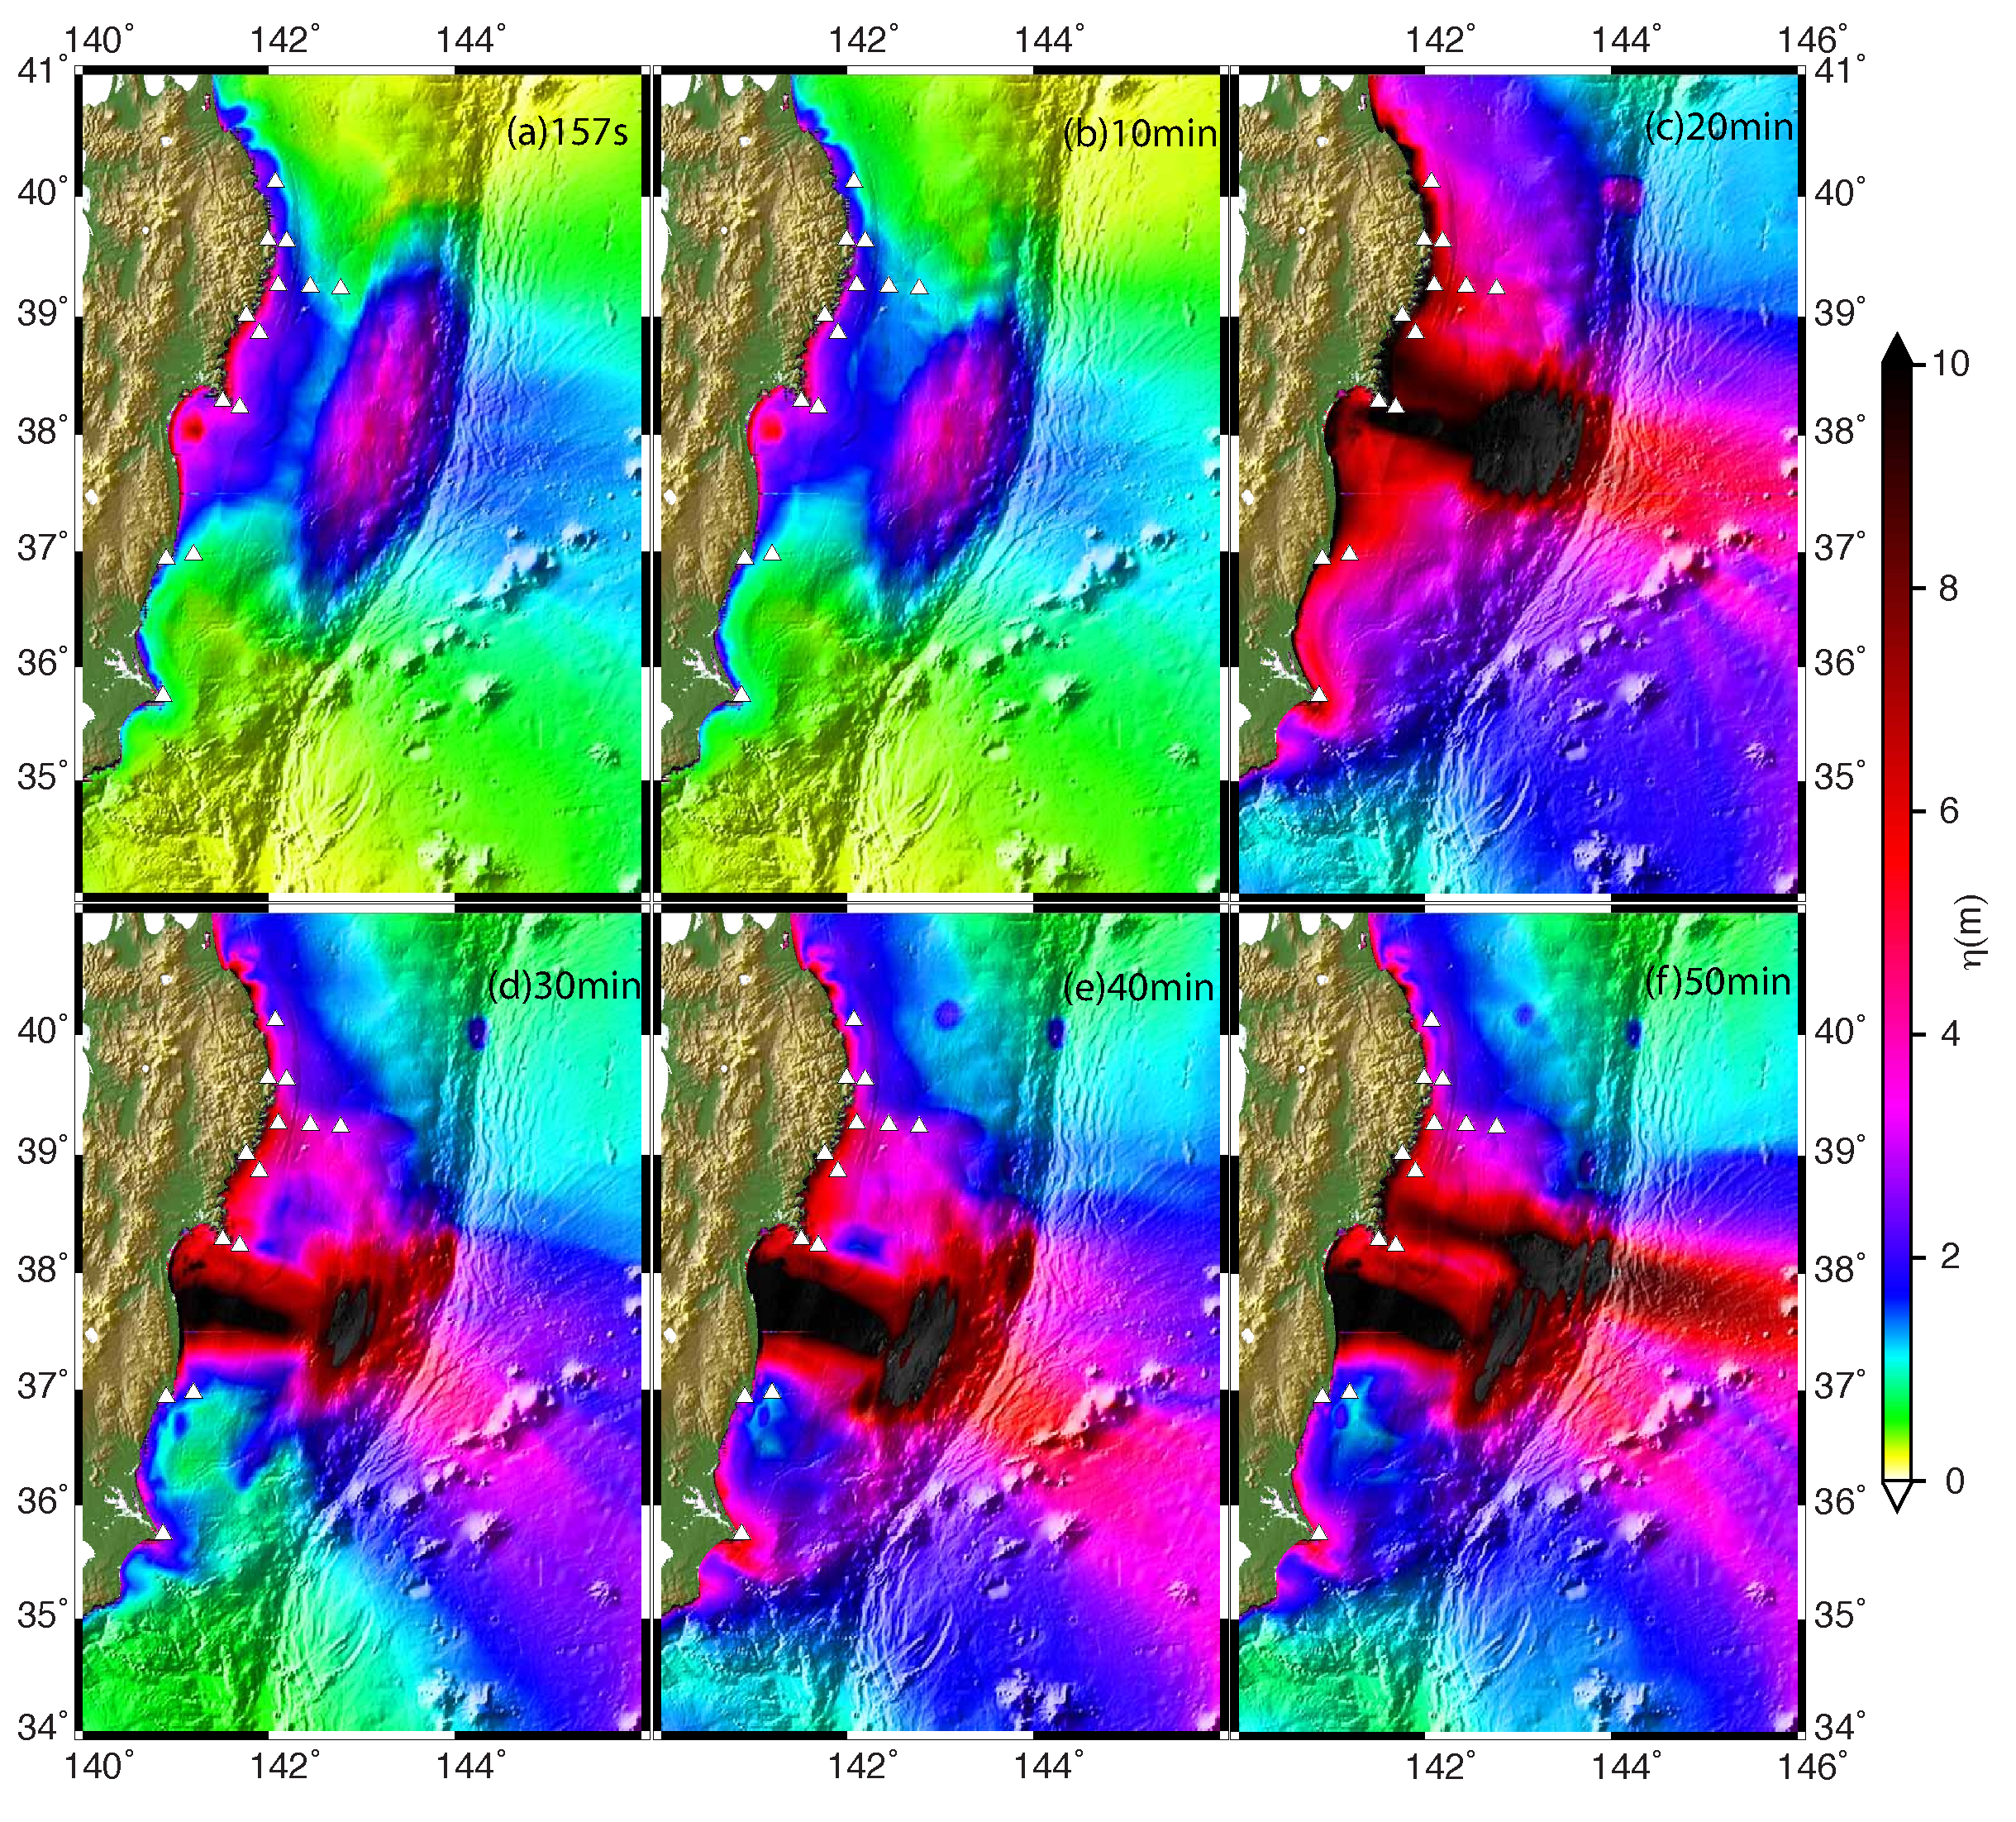
\includegraphics[width=0.9\linewidth]{./figures/ch5/inundation_all.pdf}
    \caption[Tsunami amplitude forecast results]{Tsunami forecast results. (a)-(f) Maximum expected tsunami amplitude at different intervals after earthquake origin time. The white triangles denote the positions of the wave gauges used in the joint inversion.}
  \label{fig_forecast}
\end{figure}


Figure \ref{fig_inundation} shows the inundation computed at the coast as defined by the pre-tsunami water-land boundary for each simulation. It also shows the comparison between the inundation measured by \citet{mori2012} at the survey points and the inundation predicted by our simulations at those same survey points. The first two models at 157s and 10min show a relatively smooth distribution of expected coastal inundations between 0 and 10m. They also show a systematic under-prediction of the inundation at the survey points and only 900-950 of the 2256 survey points are inundated (Table \ref{tb_results}). The variance reduction is high for these points (80-85\%, Table \ref{tb_results}). This indicates that even though many points are not inundated, those that are inundated are accurately modeled. As noted in the slip inversion (Figure \ref{fig_results1}), at 20 min the modeled sea floor deformation increases substantially and this has a noticeable impact on the inundation. The coastal inundation is now 10-20m and 1913 of the 2256 survey points are inundated (Table \ref{tb_results}). However the comparison at the survey points shows a systematic over-estimation of the inundation. This is evidenced as well by the low variance reduction of the survey inundation (59\%). Between 30 and 50min. as the slip inversion stabilizes the inundation estimates at the coast stabilize as well. The number of inundated survey points in this time interval is reduced to ~1600 out of 2256 (Table \ref{tb_results}) and the variance reduction improves to 77\% by 50min. The majority of the survey points that are not inundated by the slip inversions lie in the Sanriku coast between 38.4$^\circ$N and 40$^\circ$N.

\begin{figure}[!ht] 
  \centering
  \includegraphics[width=0.85\linewidth]{./figures/ch5/inundation_cross.pdf}
    \caption[Tsunami inundation forecast results]{Inundation forecast results. (a)-(f) the left panel shows with blue bars the inundation predicted by the model at the coastline (the pre-tsunami land-water boundary) compared to the surveyed inundation inland (orange dots). The right panel shows the direct comparison between the observed survey inundation (grey dots) and the inundation predicted by the model at the survey points (blue dots). The red crosses are survey points that were not inundated by the model. }
  \label{fig_inundation}
\end{figure}

\section{Limitations and Implications for Warning}

We have demonstrated in Chapter 3 how precise estimates of coseismic motion from seismogeodetic data could produce slip inversions of the Tohoku-oki event in about 3 min. For tsunami early warning the inundation results computed in this work show that the smooth slip inversion computed only from land data under-predicts the tsunami. However, this estimate is available quickly (157s after rupture initiation) and is a significant improvement over the initial wave height estimates that relied on the first magnitude estimate of Mw 7.9 \citep{ozaki2011}, indicating more accurate magnitude estimation and improved depiction of the geographic extent of moment release. This result is significant for more reliable early forecasts and hazard mitigation. Furthermore, the situation rapidly improves as offshore wave gauge data are ingested into the inversion. By 20min after OT the forecast of inundation (Figures \ref{fig_forecast} and \ref{fig_inundation}) shows an acute increase in intensity that better reflects the observed inundation pattern � the first waves arrived at about 30min after OT. This could in an operational setting lead to a revised warning with higher predicted intensities. By 30min a solution, which can be considered final, is available and it successfully predicts most of the gross features of inundation. This is most significant for rapid response by providing an improved determination of the hardest hit areas.

As noted by \citet{arcas2012} the multiplicity of possible earthquake source models that arise by virtue of the non-uniqueness of the inversion pose a challenge to forecast and warning. The results discussed here convincingly demonstrate that in spite of this, the objectively determined slip inversions discussed herein can replicate the pattern of inundation with minimum assumptions. We have quantified the models� skill by comparing to inundation measurements. We also argue that coseismic offset estimates (land-based data only) can serve to initiate response for tsunami early warning. Additionally, and perhaps more importantly, these results demonstrate that wave gauges in relatively shallow water ($\sim$100-1000 m) can be successfully employed to determine the earthquake source and forecast the ensuing tsunami. One need not deploy the sensors in deep water to allow for successful forecast of tsunami intensity. It remains true however, that the non-linearity in tsunami propagation exists. It is manifested most strongly in shallow tide gauge stations and at longer times after the first arrival, limiting their utility. In light of this and the discussion on linearity in Section \ref{sec:linearity}, when performing a joint inversion, it would be ill-advised to use long segments of the wave gauge records after the first arrival. Furthermore, before performing a joint inversion at other locations and with other wave gauge data one must exercise due diligence and ascertain that the non-linearities are indeed small. However, that shallow water wave gauges can be used for warning is an important result. The time taken to obtain a solution that forecasts a tsunami of the observed intensity (20min) is a function of the distribution of such wave gauges. Figure \ref{fig_forecast} shows that the distribution of such stations is not optimal for observation of this particular event. It remains possible that the forecast and warning timeline will continue to diminish as such networks of sensors become denser. GPS buoys are particularly attractive. In their current mode of operation they rely on baseline positioning and are referenced to a GPS station on-shore. This limits how far off-shore they can be deployed ($\sim$20-30km) without losing accuracy and also means that if the reference station moves, as was the case with this large earthquake, then the position solution at the buoy will be degraded. However, recent advancements in precise point positioning and tightly coupled Kalman filtering with accelerometers \citep{Geng2013} show that it is possible to do away entirely with the nearby reference station and retain the same level or even improve the precision obtained with relative positioning. This makes it possible to deploy GPS buoys at arbitrarily large distances offshore only limited by telemetry considerations.

The results and analysis shown here have some limitations and it is important to understand them. In the linear inverse framework we have sacrificed some of the fit to the coseismic data (Table \ref{tb_results}) to fit the tsunami data as best we can, especially, the ocean bottom pressure and GPS buoy stations. The general pattern of coseismic deformation is still modeled and provides a valuable constraint. However, the fit to the coseismic data is reduced from 99\% variance reduction in the land-based inversion to $\sim$~70\% levels in the joint inversion. As noted by \citet{hill2012} this can be ameliorated by placing slip where the model resolution of coseismic offsets is the lowest. This effectively locates the slip in the null-space of the coseismic data and hence doesn�t affect the data fit. We are exploring these null-space techniques and assessing their utility for real-time algorithms. Additionally, the short-wavelength along-strike features in the computed vertical deformation (Figure \ref{fig_results1}) are an artifact of the fault discretization. Very shallow subfault patches have such peaked vertical deformations that if discretization is not fine enough (our subfaults are 25x25 km) this behavior arises. This is a common problem in inversions that allow slip to go to the trench axis while keeping subfault size constant along the slab model. Given the good fits to the tsunami wave gauges we do not consider this a substantive issue for rapid computations. Future improvements to the inversion techniques might include employing irregular grids to allow for finer discretization at shallow depths. We are however interested in a speedy computation so we have chosen to keep the discretization at its current coarseness.

\citet{macinnes2013} noted that tsunami simulations from different geophysical data sets and techniques failed to capture the large inundation levels observed in the Sanriku coast between 38.4$\circ$N and 40$^\circ$N. Although we can forecast large inundation amplitudes in Sanriku we observe a similar pattern. It is noteworthy that inversions that directly employ wave measurements, like ours, fail to completely model the intricacies of the inundation. We believe that in large part this is due to limited resolution in the publicly available topography ($^\sim$90 m pixels) and bathymetry ($^\sim$1 km pixels) data sets used in this study. Consider Figure \ref{fig_TRIsanriku} where we compute the terrain ruggedness index (TRI) \citep{riley1999} of the topography/bathymetry grid. TRI is the mean difference between elevation at a pixel and its neighboring 8 pixels. The geomorphic features of the Sanriku coastline are characterized by rias, which are rugged and steep coastal inlets made from submergence of fluvial valleys. The Sanriku region has the most instances of inundation survey points that are not wetted by our simulations. 

\begin{figure}[!ht] 
  \centering
  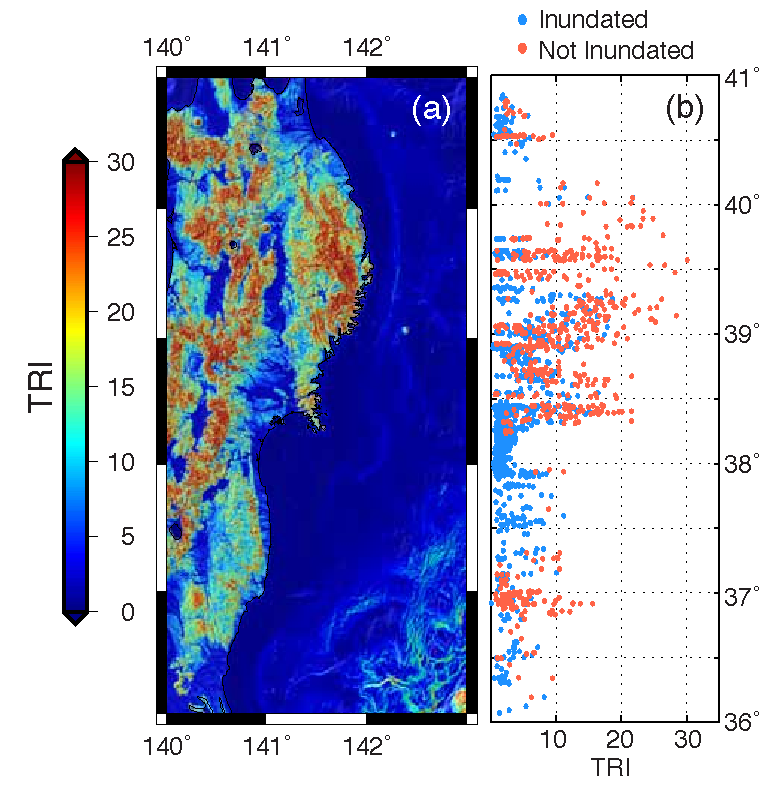
\includegraphics[width=0.8\linewidth]{./figures/ch5/TRIsanriku.pdf}
    \caption[TRI along the Sanriku coast]{(a) Terrain ruggedness index (TRI) of the topography/bathymetry grid used in this study. (b) Distribution of inundated and non-inundated survey points for the simulation at 50min after OT as a function of TRI.}
  \label{fig_TRIsanriku}
\end{figure}

	Figure \ref{fig_TRIsanriku}a shows that indeed this region has the largest TRI. Also of note in Figure 9\ref{fig_TRIsanriku} is that at the coastline in Sanriku the TRI drops abruptly from $\sim$30m on the landward side to 0m on the seaward side. It is unlikely that such abrupt change of geomorphology at the waterline is real; the rias should continue offshore forming significant underwater canyons. More likely is that because the bathymetric portion of the grid has a lower resolution (30 arcseconds, as opposed to 3 arcseconds onshore) it fails to resolve the jagged offshore features associated with rias. Figure \ref{fig_TRIsanriku}b shows the TRI values of the topography pixels containing the inundation survey points. It shows the TRI values for survey points that are wetted by the simulation and for those that remain dry (i.e., where the simulation fails to model an inundation) for the final run obtained with the data accrued at 50 min after OT. We can see from this plot that although the simulation inundates some of the survey points with high TRI, most of the survey points that remain dry have consistently high values of TRI. This can be best seen in Figure \ref{fig_TRIhist} where we bin the dry/wet survey points in 2.5 TRI intervals. It is clear, that with increasing terrain ruggedness, the model fit diminishes. Thus we believe that terrain complexity not captured by the grids is an important factor. One way to improve the capacity of earthquake source models to accurately forecast the inundation is to employ better quality grids in regions of high TRI. GeoClaw can easily handle this without a prohibitive increase in computation time with its adaptive mesh refinement approach, but currently such datasets are proprietary. 

\begin{figure}[!ht] 
  \centering
  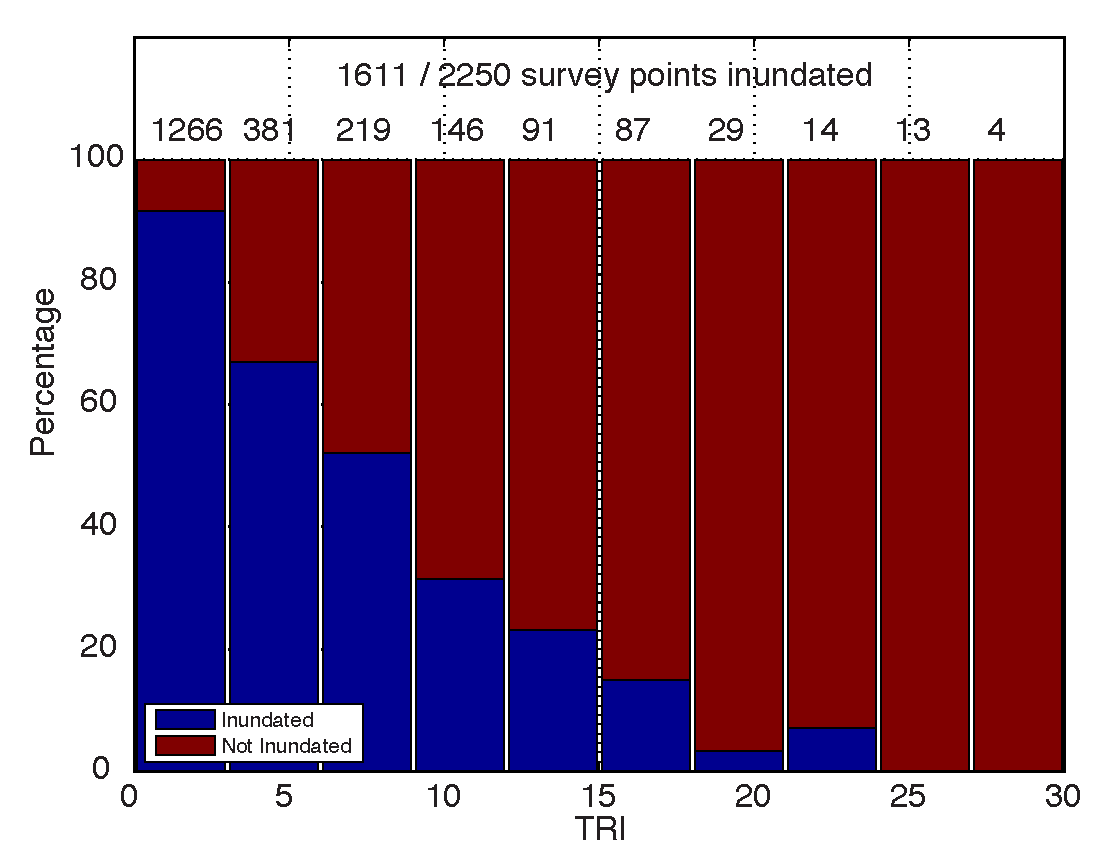
\includegraphics[width=0.7\linewidth]{./figures/ch5/TRIhist.pdf}
    \caption[TRI histogram]{Inundation of the survey points for the model obtained at 50min after origin time. This is the distribution of survey points by terrain ruggedness index (TRI) binned every 2.5 units. The number above the bar is the total number of survey points in that bin. The blue portion of the bar represents the inundated points and the red represents the fraction that is not inundated by the simulation.}
  \label{fig_TRIhist}
\end{figure}

It is also important that early warning systems be coupled with judicious analysis of the hazard before an event occurs. For example, pre-event analyses with better bathymetry would undoubtedly show that a 10m tsunami at the mouth of a ria, as in the Sanriku coast, could be greatly amplified by the local bathymetry. Thus even if the first estimation of tsunami intensity (Figure \ref{fig_inundation}a) is an underestimate, coupling with a priori knowledge of the hazard can lead to a better response. Warning is only one part of the response system. Pre-event analysis of the hazard and societal education are just as important, and without them a warning is of little use.

Additional close inspection of the GPS buoy records (i.e. Figure \ref{fig_results2}g) shows that all models underestimate the peak tsunami amplitude at the northernmost buoys, BY.IWC and BY.IWN (Table \ref{tb_wave_stations}). This is one of the regions of higher TRI. Nearby BY.IWS and tide gauges TI.OFU and TI.MYO are well modeled although the tide gauge records are clipped and we are unable to say if maximum amplitude would have been correctly modeled. We also note that the final source model consistently places a streak of 5-10m of slip on the northern portion of the fault at around 40$^\circ$N. These two observations (the underestimate at the northern buoys and the streak of slip on the northern part of the model) imply that we cannot discard the possibility that secondary sources of tsunami energy \citep{morra2013} (i.e., submarine landslides, splay faults, etc.) are contributing to the wave records and contaminating the inversion results. Quantifying and modeling the contributions of such sources to the overall radiation pattern of the tsunami remains a challenge to early warning and tsunami science in general. It is possible that other assumptions lead to the observed discrepancy. For example GeoClaw does not consider the contribution of horizontal momentum to tsunami generation. It is possible that motion of large vertical features such as continental slopes might have an important contribution to the tsunami energy budget. Only recently has this assumption been seriously studied \citep{satake2013}. Additionally, in tsunami modeling it is customary to assume instantaneous tsunami generation. For example, for the 2004 Sumatra event it was shown that time dependent rupture models had little effect on the observed tsunami \citep{fujii2007}. However \citep{satake2013} argues that for Tohoku-oki, near-source observations are best modeled with a kinematic slip model. Part of our future research is to employ near-field broadband strong motion displacement data recorded for this event [Melgar et al., 2013a] and wave gauge data to derive kinematic models. It will be important to assess the impact of such techniques on rapid tsunami response.

The Japanese GPS network (GEONET) is very dense and its inter-station spacing an exception rather than a norm worldwide. In this study we used a sparser subset of 139 stations (the collocated GPS/accelerometer pairs) to compute the first inversion. This was done to demonstrate the capabilities of the seismogeodetic solution and also to illustrate the performance with a station distribution more akin to other regional GPS networks. We found that the sparse seismogeodetic solution is adequate and can be computed quickly but in general it underestimates the inundation. The effect of this undersampling the land-based network is illustrated in Figure \ref{fig_allgeonet} where we present the inundation predicted by the optimal inversion resulting from employing the displacement waveforms from the 816 GEONET stations in the affected region. The maximum amplitude forecast is larger than in the seismogeodetic solution alone and closer to the result from the joint inversion. The comparison with the survey points improves, 1538 out of the 2250 survey points are inundated by the full GPS network solution and variance reduction is 70\%. Not surprisingly, a denser land GPS network provides a better early forecast of the tsunami and would be further ameliorated by collocation with accelerometers at all stations. In general, the methodology described herein can be employed with GPS data alone, however we've shown that the improved vertical resolution resulting from the seismogeodetic combination improves the derived finite fault slip model. Furthermore, the prospect of real-time coseismic source modeling with corrected strong motion records alone remains elusive.

\begin{figure}[!ht] 
  \centering
  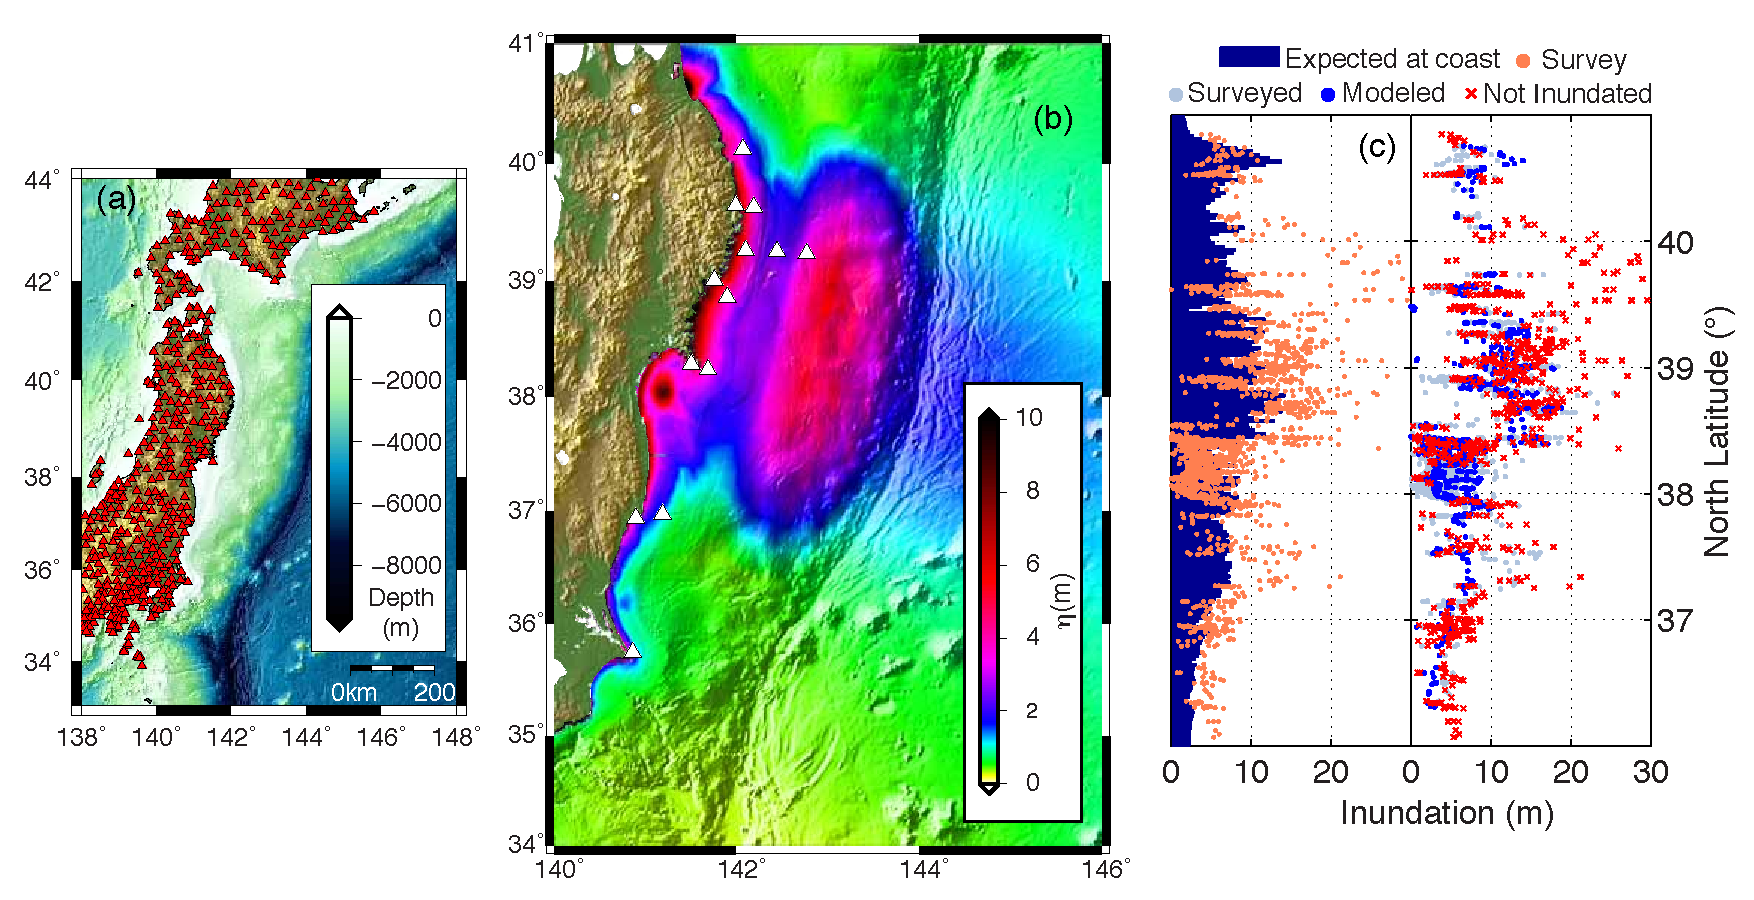
\includegraphics[width=0.99\linewidth]{./figures/ch5/all_geonet.pdf}
    \caption[Inversion with dense GEONET stations]{Inundation results at 157s after OT from the inversion employing the dense 816-station GPS network. (a) Outline map of the station distribution; (b)  Forecast of maximum expected amplitudes; (c) Inundation results as in Figure \ref{fig_inundation}.}
  \label{fig_allgeonet}
\end{figure}

Although in this work we have focused on the immediate impact of the tsunami, i.e., the inundation, the time evolution of the models shows that there is significant structure to the tsunami even hours after origin time. This can have important impact on coastal and ship operations \citep{lynett2012}. Thus longer-range forecasts could be aided by the results discussed here.

We also note that the algorithm employed in this study relies on the traditional method of regularization to solve an ill-conditioned inverse problem. The results are encouraging and driven by the requirement of rapid computation. Inversions for 200 distinct sources at different smoothing levels takes only a few minutes on a four-core machine and are easily parallelizable since each inversion is independent of all the others. Nonetheless the issue of selecting the smoothing parameter automatically and objectively remains irksome. We have employed the statistical argument of minimizing information loss by using the ABIC. However, we foresee that as computational power increases it will become feasible to use fully probabilistic techniques to determine the earthquake source \citep{minson2013}. Such Bayesian approaches are desirable because they sample all models that are consistent with observations while restricting the ensemble to those that fit the assumptions about the underlying physics. This is preferable over solutions that require regularization or smoothing which is, in a sense, an artificial numerical restriction not strictly based on a tangible physical constraint. Such Bayesian algorithms are currently burdensome because of the large number of free parameters involved in computing the earthquake source. Recently these approaches have become more computationally tractable with better sampling techniques [Minson et al., 2013] but not yet to the degree where they can be computed immediately after the earthquake origin with ease. However, the advances are promising. In this probabilistic paradigm one can produce rapid estimates of hazard curves along the coastline \citep{gonzalez2009} instead of point estimates of inundation intensity. One could then more adequately characterize the hazard and contemplate the creation of higher-level products such as expected economic impact and rapid loss calculations similar to what the PAGER product does for earthquake shaking.

This is a rapidly evolving field. Leveraging earlier results from [Melgar et al., 2013b] we have demonstrated an end-to-end automatable methodology that minimizes operator interaction. Starting with the land-based data that are available many minutes before sea-borne measurements, we determine basic source parameters, i.e., magnitude, type of faulting and geographic extent from the line source CMT inversion. This then allows selection of appropriate fault-model geometry to launch a heterogeneous finite fault slip inversion. Once the slip inversion is computed, sea floor deformation can be calculated and used as the initial conditions for a model of the tsunami. This yields a first forecast of tsunami intensity and can be used for warning. Then, as time goes on, wave gauges information is ingested and the inversion rerun. The new updated earthquake source is used to obtain a new tsunami model and forecast. For the Tohoku-oki earthquake the first forecast is available at 157s after OT. At 20 minutes after origin time a revised forecast that has high inundation amplitudes is determined; recall maximum inundation at the closest points on the coast was not reached until 30 minutes \citep{ozaki2011}. After this time (OT+30min) the earthquake source and tsunami forecasts remain without major changes. We have proposed an indirect form of forecast and warning that is much improved because it relies partly on direct measurements of tsunami wave propagation to compute the earthquake source and not just on traditional seismological measurements.

Thus, we contend that we have demonstrated that with current geophysical sensor technology and algorithms the expectation of detailed and timely tsunami forecast and warning in the coastal areas adjacent to large earthquakes, regardless of their faulting type and location, is a realistic one.

\section{Joint Kinematic Inversion of Land- and Ocean-Based Sensors}

We can incorporate the tsunami waveforms into the kinematic inversion following the same modelings steps as in Chapter 4 and Section 5.2 and study the effects on the source and tsunami propagation and inundation pattern. We compute the time dependent motion of the seafloor suing the frequency wavenumber method of \citep{zhu2002} for 1m of slip on each of the 189 subfaults. The time dependent coseismic motions of the seafloor are then used as the starting conditions for tsunami simulations in Geoclaw. We model 60 minutes of the resulting tsunami from slip on each of the sub faults at the locations of the wave gauges. These are then considered kinematic tsunami Green's functions and incorporated into the kernel matrix $\mathbf{G}$. We then follow the same approach as before and utilize Akaike's Bayesian information criterion to determine the optimal spatial and temporal smoothing for the inversion.

There is good reason for incorporating the tsunamis waveforms into he modeling process. Generally it was believed that instantaneous slip as in Sections 5.1-5.4 was sufficient to model tsunami propagation. \citet{fujii2007} found for the 2004 $M_w9.2$ Sumatra event that the tsunami waveform data was largely insensitive to kinematic models of the source. However, in that study they relied mainly on far field data. Later \citet{satake2013} demonstrated that for the Tohoku-oki case kinematic models better explained the tsunamis waveforms and inundation data of \citet{mori2012}. It is reasonable to assume that in the tsunami near-field time dependent deformation of the sea floor provides a better initial condition for propagation modeling. Following we will show the results of the joint kinematic inversion of the seismogeodetic displacement, velocity and tsunami data. \citet{satake2013} performed the kinematic inversion of only the tsunami data on a coarse 55 sub fault model and obtained 69m of slip at the trench and up to 10m of slip at depth. By incorporating the land data as well we can obtained a finer picture of the source. Furthermore, \citet{satake2013} used a totally reflecting boundary condition at the coast while with Geoclaw we can compute physically realistic tGFs that allow wetting and drying of the coastal cells in the model. Additionally, since the coastal tide gauges display non-linear behavior we will disregard them for the following models and we will retain only the 2 ocean bottom pressure gauges and the 6 RTK GPS buoys (Table \ref{tb_wave_stations}).

\subsection{Tsunami Generation by Horizontal Coseismic Motion}

Another improvement on the static modeling results of Sections 5.1-5.4 is that we will account for the tsunami generation effects of horizontal coseismic motions as well as the vertical ones. \citet{tanioka1996} recognized that steeply sloping bathymetric features subject to large horizontal motions contribute to tsunamigenesis. This effect is generally disregarded and only coseismic vertical deformation is incorporated into the tsunami source, as we did in the static modeling case. \citet{fujiwara2011} observed 50+m of horizontal motion at the trench, this encourages us to account for these effects. Figure \ref{fig_coseis_horiz} illustrates how sloping bathymetry can cause pseudo-uplift of the seafloor. 

\begin{figure}[!ht] 
  \centering
  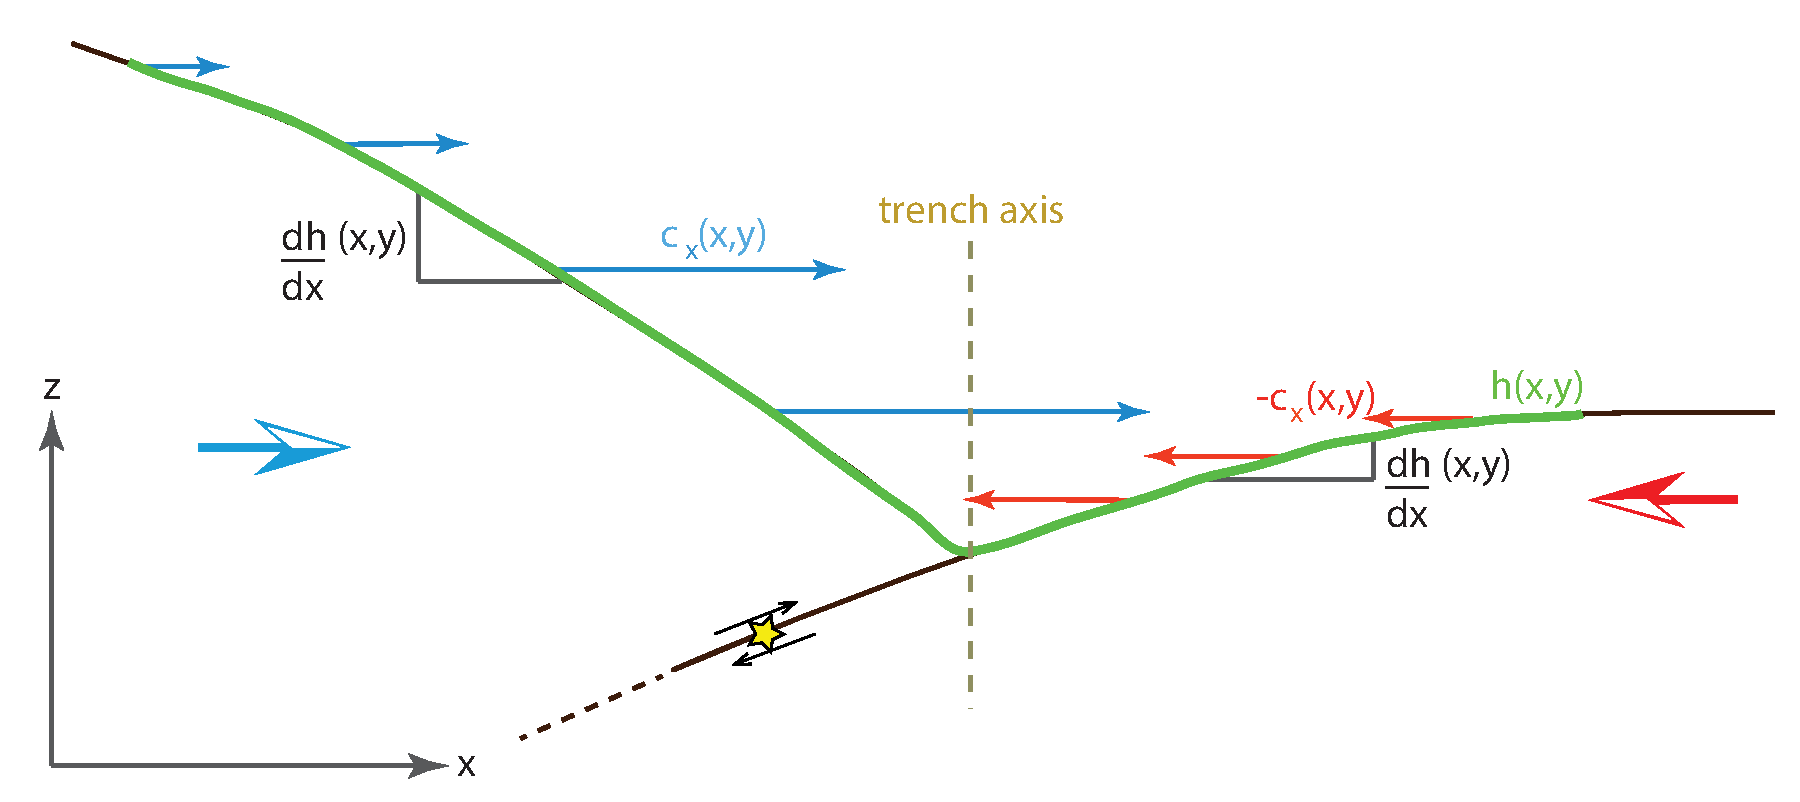
\includegraphics[width=0.99\linewidth]{./figures/ch5/coseismic_cartoon.pdf}
    \caption[Schematic of tsunami generation from horizontal motion]{Schematic of tsunami generation from horizontal coseismic motion $c_x$, see text for details.}
  \label{fig_coseis_horiz}
\end{figure}

We approximate bathymetry as a smooth function which depends on two horizontal coordinates $h(x,y)$. Slip at depth will cause horizontal motions $c_x(x,y)$ and $c_y(x,y)$ of the bathymetry in both horizontal directions. If there are sloping features in the bathymetry this horizontal deformation causes an apparent vertical motion which we can locally approximate by considering the directional derivative of bathymetry. Then the total apparent vertical deformation $\Delta  h$ will be the sum of the coseismic vertical deformation, $\Delta z$ and the horizontal one due to the motion of the sloping features such that
\begin{equation}
\label{eq:uplift}
\Delta h(x,y)=\Delta z(x,y)-c_x(x,y)\cdot\frac{dh}{dx}(x,y)-c_y(x,y)\cdot\frac{dh}{dy}(x,y)\;.
\end{equation}
Note the negative signs in front of the directional derivatives. These indicate that the downward sloping feature west of the trench axis (negative derivative) moving in the positive $x$ direction should cause uplift, as should the upwards sloping feature east of the trench axis moving in the negative $x$ direction. This differs from the initial condition we used in the static approximation where we simply have $\Delta h(x,y)=\Delta z(x,y)$. These adjustments are considered in generating the kinematic Green's functions as well as the inundation models that follow. To further illustrate the effect that the sloping bathymetry can have in vertical deformation consider Figure \ref{fig_derivative} where we show the directional derivative of the SRTM30+  bathymetry computed along the average trench-normal direction. The red colors indicate that positive horizontal motion causes uplift, while the blue ones that positive motion causes apparent subsidence. Along the frontal part of the continental slope and close to the trench the values of the derivative are as high as 0.3, the values are also high along the sea mounts south of 37$^\circ$N. This means that for every meter of horizontal motion 30cm of apparent vertical motion will be generated. Clearly, this is not a signal that should be ignored.

\begin{figure}[!ht] 
  \centering
  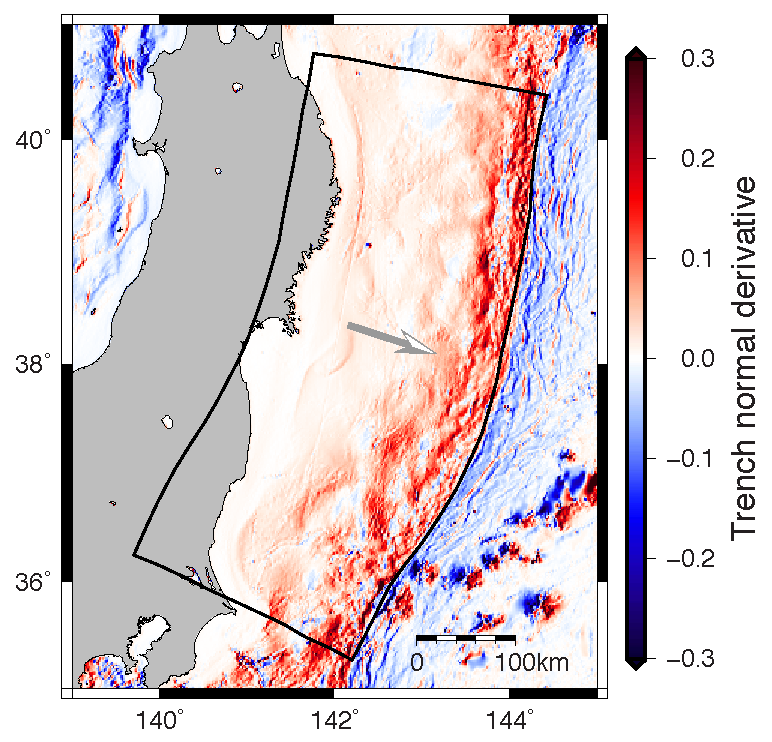
\includegraphics[width=0.8\linewidth]{./figures/ch5/derivative.pdf}
    \caption[Trench normal derivative of bathymetry]{Trench normal derivative of bathymetry computed in the direction indicated by the grey arrow. The black outline is that of the fault model used for the inversion.}
  \label{fig_derivative}
\end{figure}

\subsection{Inversion Results}

Figures \ref{fig_dvt_results} and \ref{fig_dvt_results2} show the results after incorporating the 8 wave gauge stations into the inversion procedure. Peak slip is now 63m, compared to the 52m from the land-only inversion and moment is $5.51\times10^{22}$N-m $(M_w9.09)$ compared to $4.89\times10^{22}$N-m ($M_w$9.06) for the land-only inversion. The final slip of the land-only model (Figure \ref{fig_dvt_results}a) prefers a horizontally symmetric slip distribution about the hypocenter. For the joint inversion (Figure \ref{fig_dvt_results}b) slip is 25m or larger for the top 20km of the fault only south of the hypocenter while north of the hypocenter large slip is confined to the shallowest 10km. There is also a notable shallowing of peak slip in general with the joint model having a larger accumulation of shallow slip. The total source time functions (Figure \ref{fig_dvt_results2}a) are very similar. Peak moment rate is delayed in the joint model from 75 to 80s but its value is unaltered. Furthermore, the joint model has an increase in moment relative to the land-only model at times after peak moment rate although the total duration is similar (190s). A notable difference between both slip inversions are the two patches of 10m of slip on the shallowest portions of both northern and southern extremes. While the land-only inversion does have slip at the edges of the model (about 5m) there is a visible increase of slip in the joint model. The fits to the wave gauge data are good (VR is 71\%) (Figure \ref{fig_dvt_results2}b), notably the peak amplitudes at both pressure gauges (OB.TM1 and OB.TM2) are well modeled. As in the static case we note that the northernmost buoy (BY.IWN) shows the poorest fit between data and synthetics.

\begin{figure}[!ht] 
  \centering
  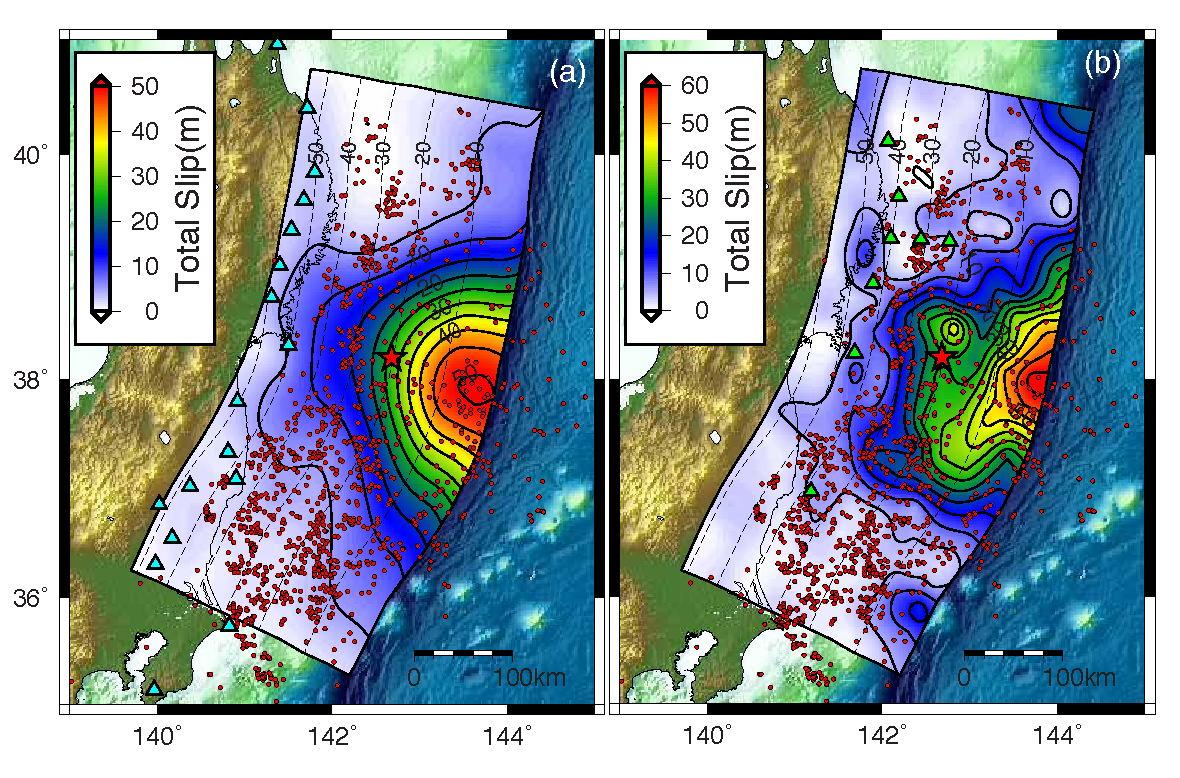
\includegraphics[width=0.9\linewidth]{./figures/ch5/dv_dvt_compare.pdf}
    \caption[Joint land- and ocean-based data inversion results 1]{Joint land- and ocean-based data inversion results. (a) Is the preferred result from the inversion of seismogeodetic displacement and velocity waveforms (Chapter 4). Triangles are the land stations, red dots are 2 weeks of aftershocks and the star is the hypocenter. Slip is contoured every 5m and depths to the slab every 10km. (b) Is the result after incorporating the 8 wave gauge stations denoted by triangles. Red dots are 2 weeks of aftershocks and the star is the hypocenter. Slip is contoured every 5m and depths to the slab every.}
  \label{fig_dvt_results}
\end{figure}

\begin{figure}[!ht] 
  \centering
  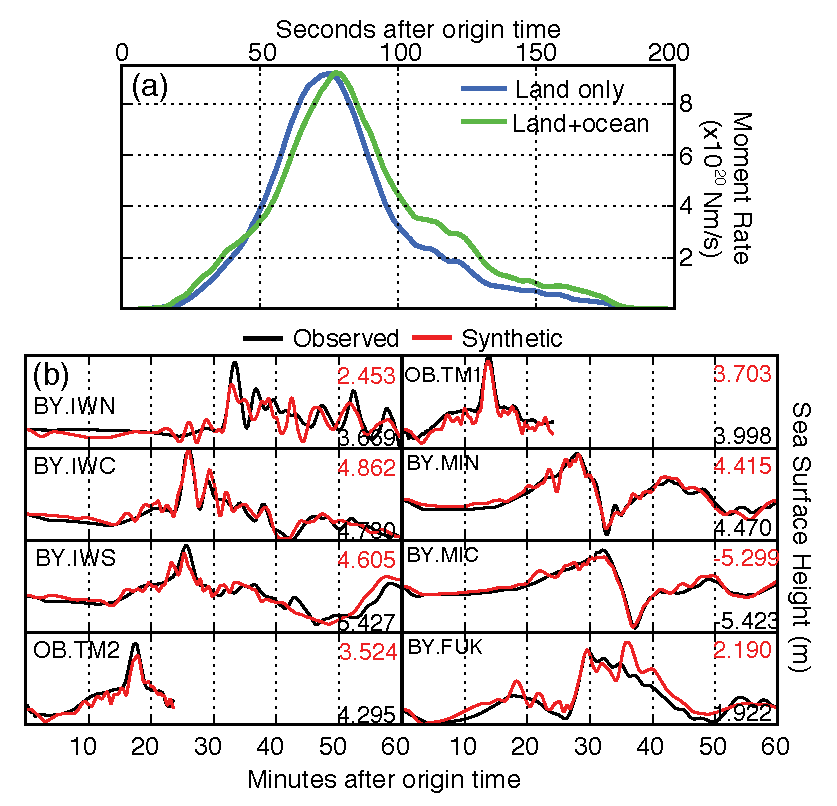
\includegraphics[width=0.5\linewidth]{./figures/ch5/dv_dvt_compare2.pdf}
    \caption[Joint land- and ocean-based data inversion results 2]{Joint land- and ocean-based data inversion results. (a) Is the comparison between the source time functions of both inversions. (b) Is the fits to the wave gauge data. The black lines are the observed and the red the synthetics. The numbers denote peak amplitudes}
  \label{fig_dvt_results2}
\end{figure}


As before we can also study the individual subfault source time functions (Figure \ref{fig_dvt_tiles}). Recall that plotted is the moment rate for every subfault with their respective 90\% confidence intervals (CIs). The white lines indicate the lower bounds of the 90\% CIs and the grey hatched areas the upper bound of the CI. The STFs are colored by pseudo-rupture velocity. This coloring indicates how fast a rupture front would have to travel to each that subfault at a particular instant in time. A comparison with the solution from Chapter 4 (Figure \ref{fig_tiles}) shows that the model is largely unchanged for the subfaults down-dip from the hypocenter. There seem to be at least two pulses of slip, the first one has low peak moment and very short durations. The second pulse propagates down dip from the hypocenter and then spreads laterally quite quickly, it has longer durations (about 20s) and higher moment rates. 

Up dip the behavior in the joint model is different from the model in Chapter 4 (Figure \ref{fig_tiles}). As we noted in the total slip distribution from Figure \ref{fig_dvt_results}b moment release north of the hypocenter is smaller. More importantly the source time functions are significantly longer for the shallowest 2 rows of subfaults and north of the hypocenter (along strike indices 5-9). In the preferred model from Chapter 4 those shallow source functions had durations of the order of 50s, while in the joint inversion here the STFs can be as long as 100s, essentially occupying the entire allowed duration. South of the hypocenter on the shallow sub faults duration of the STFs does not increase as much, but there is a second pulse of slip in the sub faults with largest moment release (along-strike indices 10-12) whose amplitude is larger than in the preferred model of Chapter 4. Overall, the effect of including the tsunami data is to produce a more pronounced pattern of shallow slip, to shift more of the moment release to the southern half of the slab model and to produce longer duration STFs on the shallowest subfaults.

\begin{sidewaysfigure}[p]
    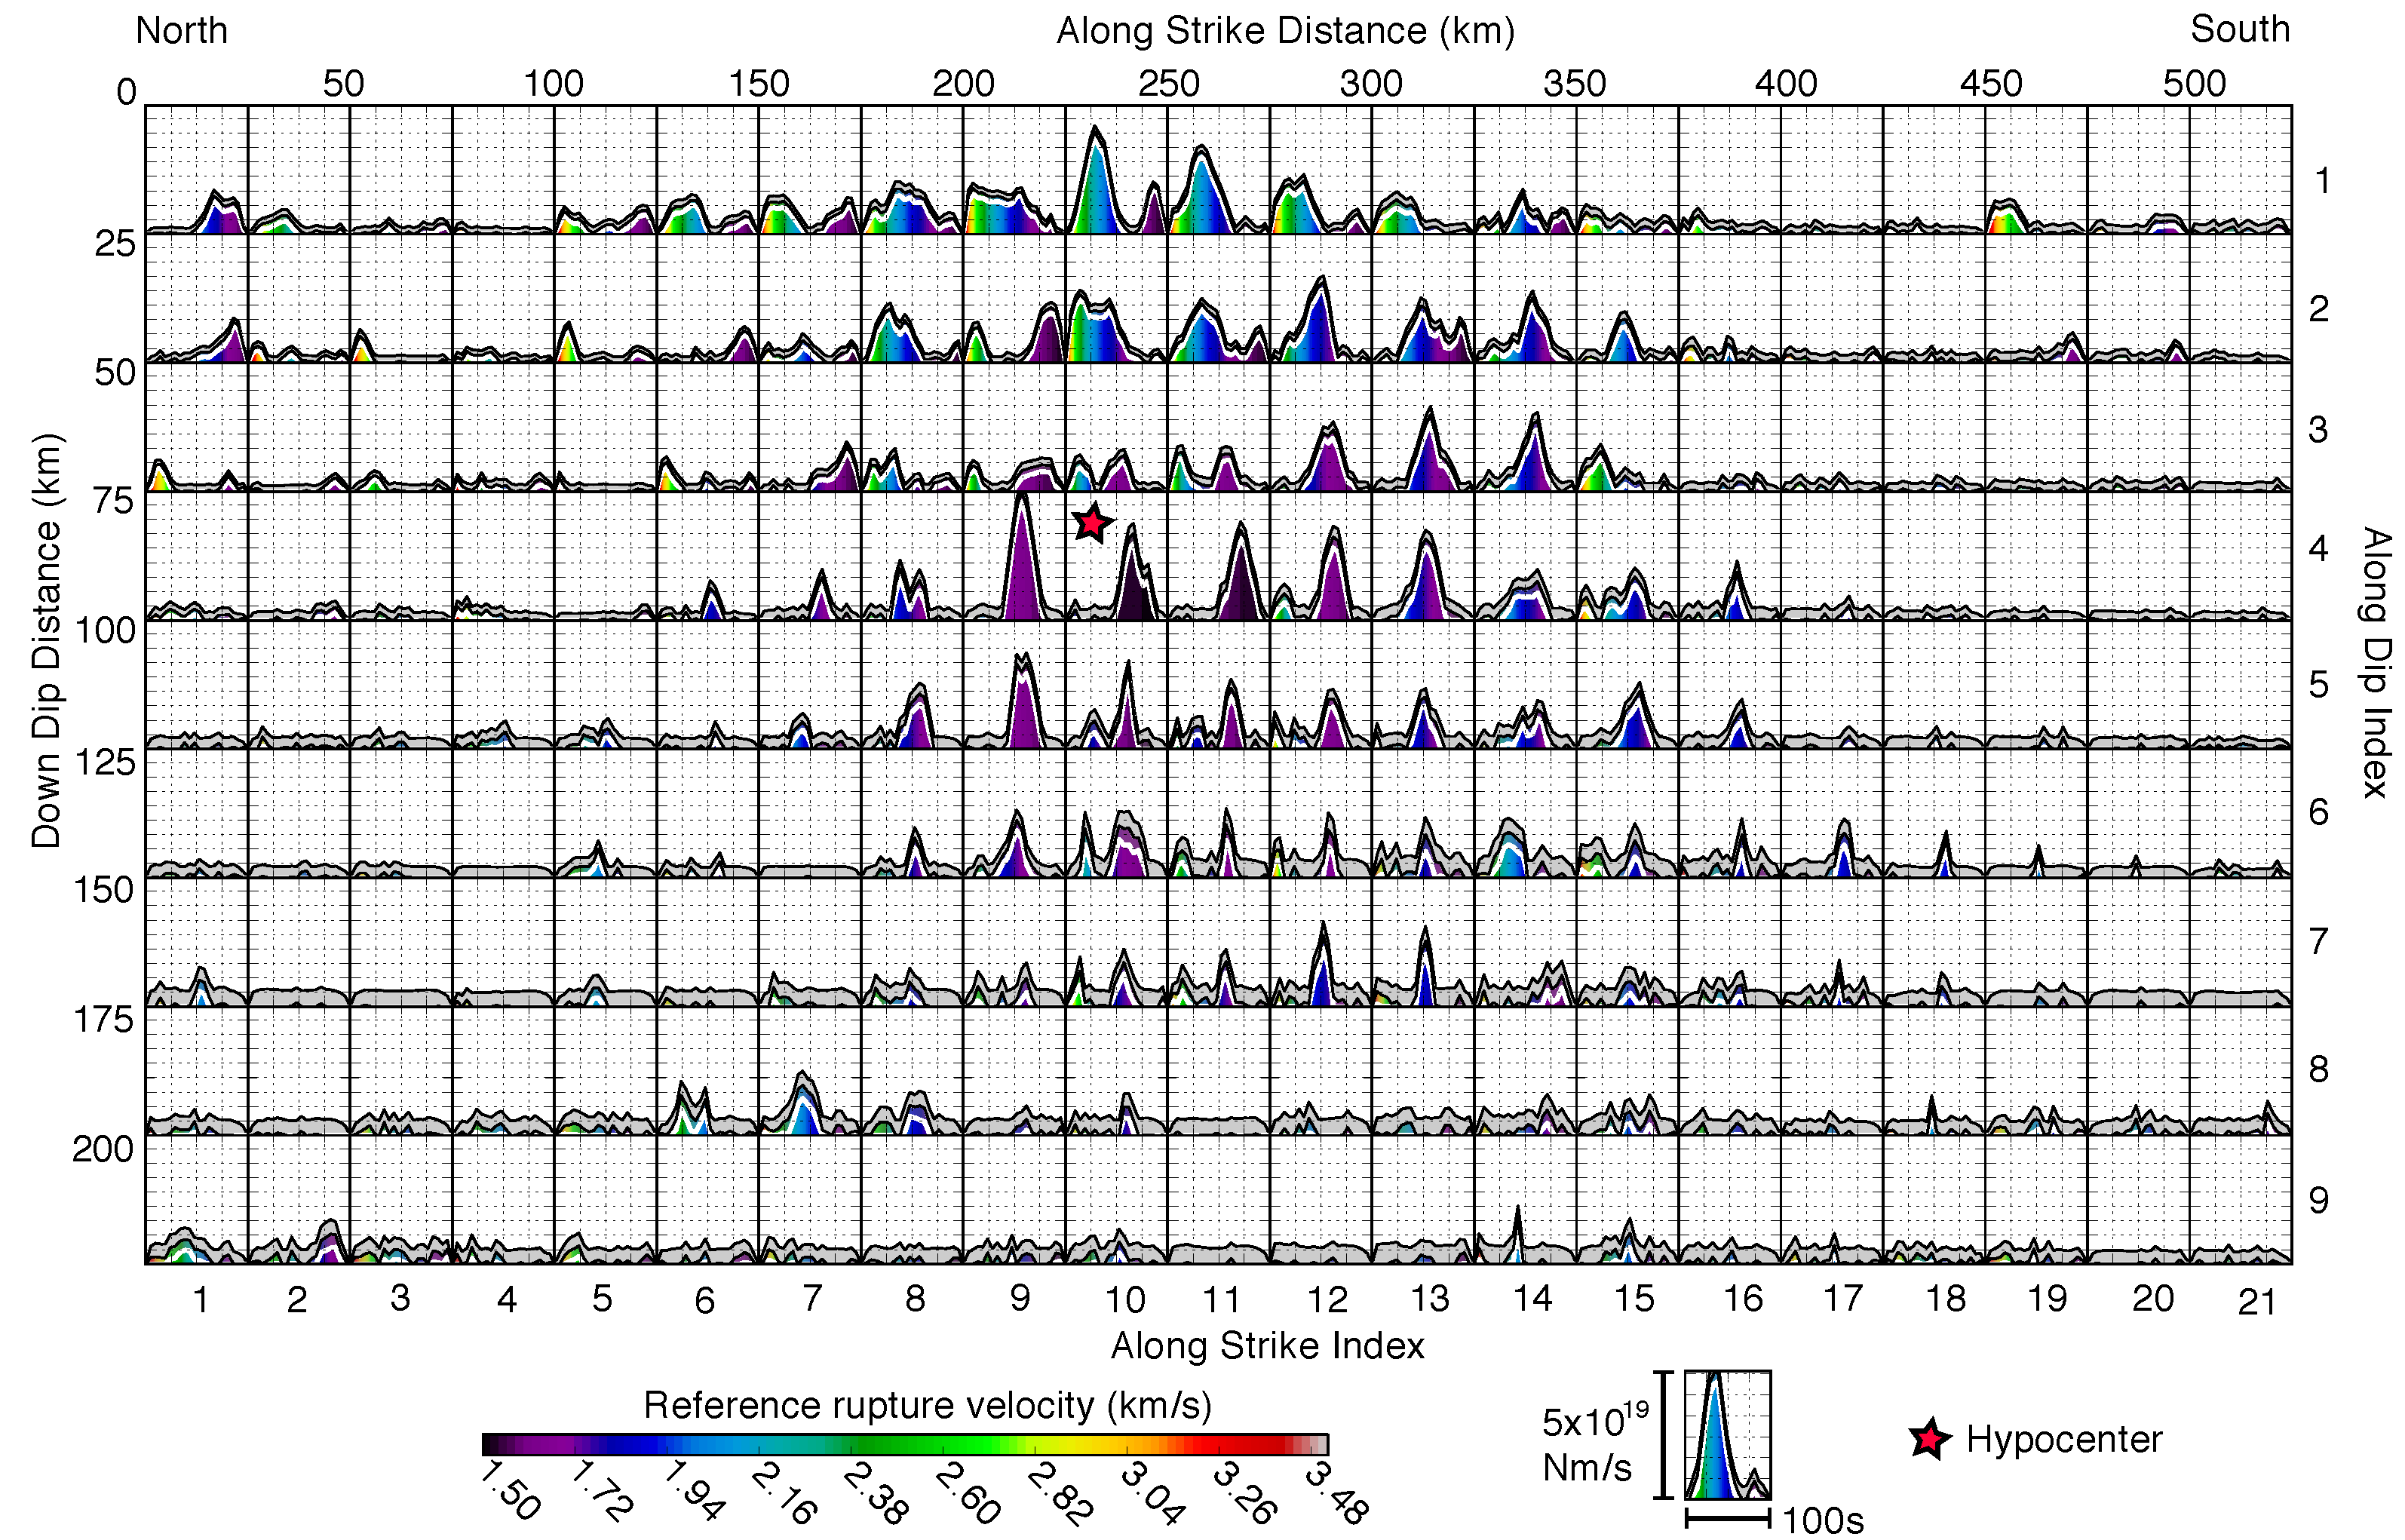
\includegraphics[width=22cm,height=14cm]{./figures/ch5/tiles_dvt_small.pdf}
    \caption[Subfault source-time functions]{Subfault source-time functions (STFs). The 90\% confidence intervals are indicated by the white line and the solid grey hatched area. The coloring under the STFs represents the pseudo rupture velocity. The red star indicates the hypocenter. All STFs are plotted at the same scale.}
    \label{fig_dvt_tiles}
\end{sidewaysfigure}

Static inversion with tsunami data has been performed before here (Sections 5.1-5.4) and by other authors \citep{fujii2007,gusman2012,romano2012}. Additionally, it has become routine to adjust geodetic \citep{hill2012} and seismic source models \citep{simons2011,lay2013} iteratively until they fit observed tsunami waveforms or inundation observations. Kinematic inversion is only a recently demonstrated possibility \citep{satake2013} with tsunami waveforms and the joint inversion with land-based data has not, to our knowledge, been performed before. As we've discussed in Chapter 4 down-dip of the hypocenter our results are consistent with other seismic slip inversions and with back projection studies. Up-dip our results are wholly consistent with the tsunami-only inversions of \citet{satake2013} they observe a similar two step slip pattern with equally long rise times. These extended slip durations at shallow depth are intriguing. The shallower portion of the megathrust is expected to have low friction material \citep{lay2012} and drilling results support this for Tohoku \citep{fulton2013}, this will result in long STFs \citep{kanamori2004}, however the seismogeodetic data in no way require STFs as long as observed with the inclusion of tsunami data. No matter the amount of smoothing applied we do not observe this. It is unclear whether the tsunami data themselves are sensitive at temporal scales of tens of seconds to changes in source duration and further sensitivity and resolution studies are necessary to ascertain whether these long slip durations are a robust feature. The patches of large slip at the northern and southern extremes of the fault model are also observed by the tsunami-only inversion of \citet{satake2013}. Note from the aftershock distribution in Figure \ref{fig_dvt_results}b that the main asperity produces a significant number of events in the outer rise, most of them normal faults \citep{asano2011}. However, in the outer-rise of the two higher slip patches at either extreme of the fault model there is no aftershock activity. This raises the possibility that those are artifacts introduced by the tsunami data. If there are secondary and unmodeled sources of tsunami energy these will be mapped onto the slip inversion. It is quite likely this is the case and future improvements will include a more physically realistic tsunami source. For example \citet{kawamura2012} documented compelling evidence from underwater cameras for mass wasting offshore Sanriku. \citet{arai2013} also demonstrated from ocean bottom pressure sensor data, heat flow measurements and cores the existence of wide-spread turbidity currents in the northern region of the Tohoku-oki source; these could very well contribute to tsunami genesis. Additionally \citet{tsuji2013} found extensive extensional faulting with measurable vertical motion in the overriding crust landwards of the continental backstop. \citet{grilli2013} also showed with 3D finite element modeling that using realistic earth structure models can improve models of tsunami generation while \citet{ma2013} demonstrated that inelastic behavior of the wedge can also significantly alter the vertical deformation pattern of the shallowest portion of the megathrust environment. The tsunami waveforms are likely sensitive to most if not all of these phenomena and it is possible that some of the differences between the land-only and the joint models arise as a consequence of this. Nonetheless, and overall it seems that inclusion of the tsunami data produces a slip pattern with significantly more detail in the shallow portion of the megathrust than previous studies have been able to resolve.

\subsection{Tsunami Modeling Results}

When employed as an initial condition for tsunami modeling, the kinematic inversion result of Figures \ref{fig_dvt_results} and \ref{fig_dvt_tiles} has a significant effect on the tsunami intensity and propagation pattern. Figure \ref{fig_dvt_uplift}a shows the total vertical deformation including the contribution of the horizontal motion of bathymetry. There is a broad region around the epicenter of long wavelength uplift between 0 and about 7m which is largely responsible for the first pulse of tsunami energy observed at the wave gauges (Figure \ref{fig_dvt_results2}b) as a slow and steady increase in sea-surface height. At the frontal part of the continental slope and particularly at the trench we have much larger uplift with shorter wavelength features (up to 22m of uplift). This deformation is associated with the short wavelength high amplitude tsunami peak which is especially visible on stations OB.TM1 and OB.TM2 at 14 and 18 minutes after origin time respectively. It is interesting to note that both deep slip and shallow slip contribute to tsunamigenesis. It is also important to remark on the contribution of horizontal motion of bathymetry to the uplift pattern. Figure \ref{fig_dvt_uplift}b shows the contours of eastward horizontal displacement predicted at the seafloor and the associated predicted uplift computed using Equation \ref{eq:uplift}. The uplift is largest in the regions of largest horizontal motion and steepest terrain (Figure \ref{fig_derivative}), namely closest to the trench (up to 3m), making this an important contributor to the tsunami initial condition. On the continental shelf as expected horizontal motions contribute very little to the vertical deformation pattern. These results agree all with the predictions of \citet{tanioka1996} who argued that horizontal motions could account for a significant portion of the tsunamigenic uplift.

\begin{figure}[!ht] 
  \centering
  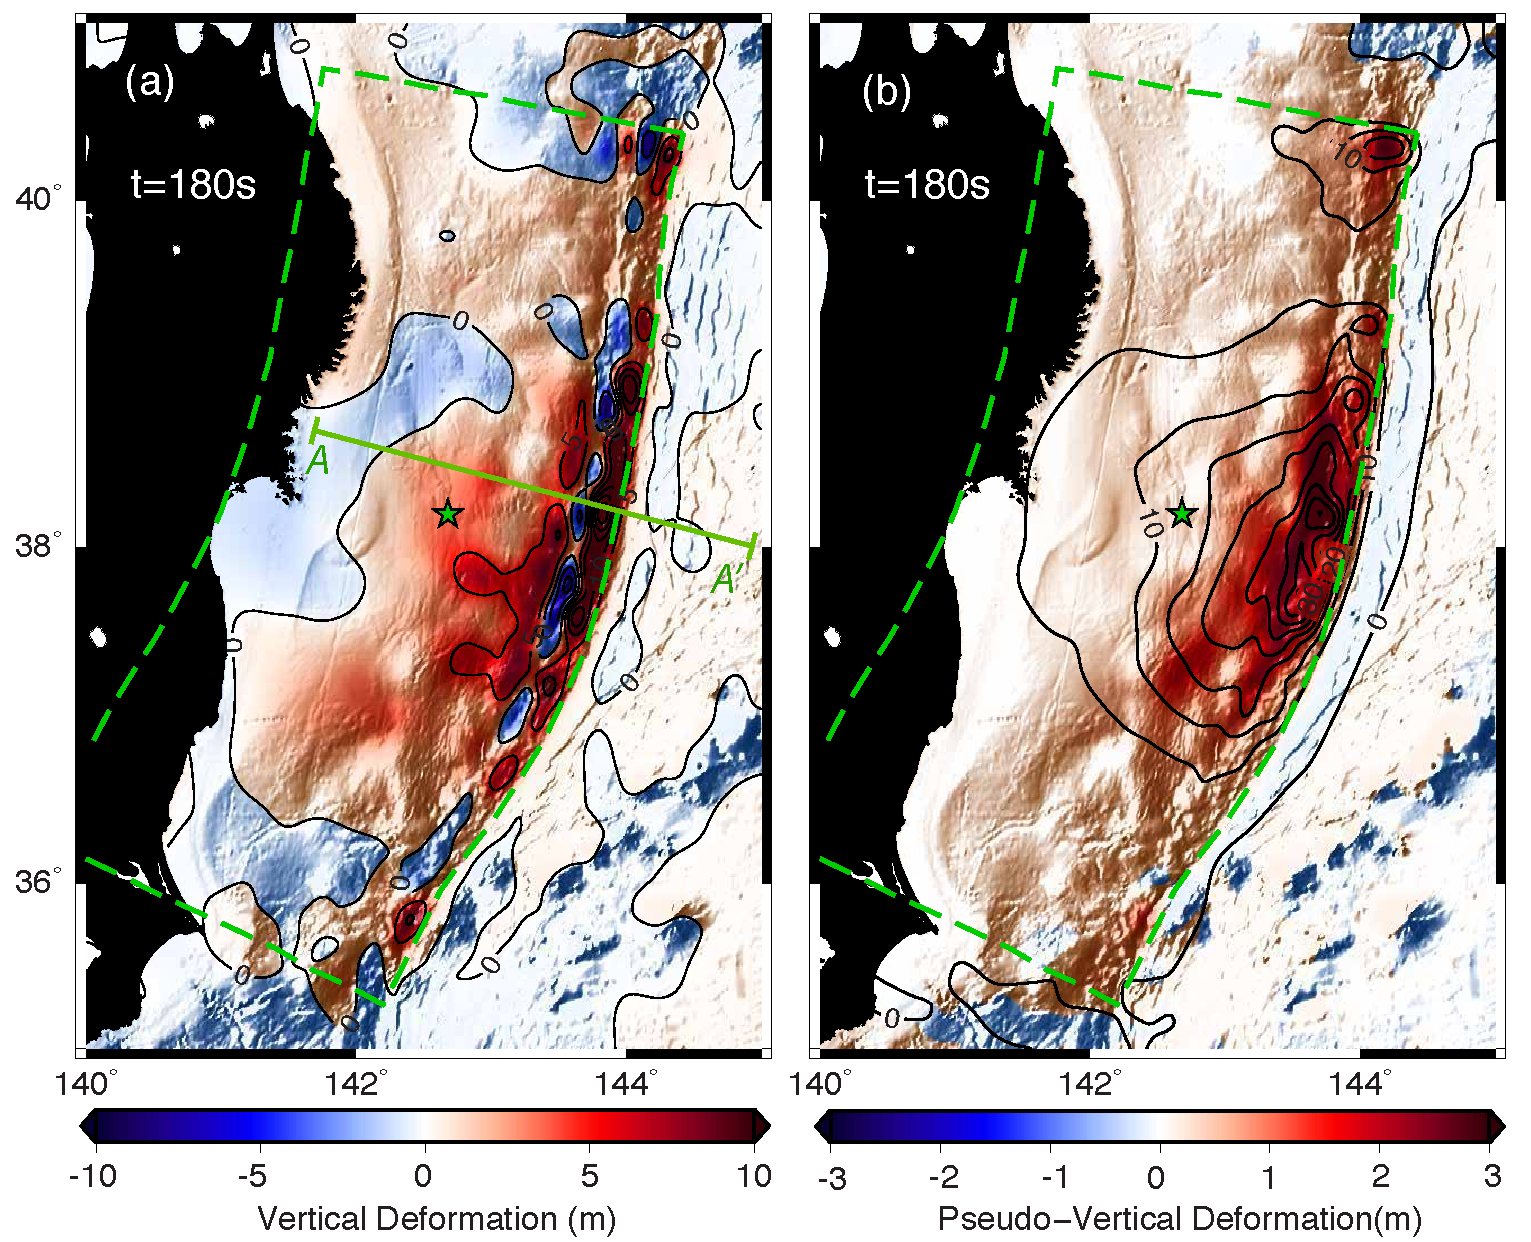
\includegraphics[width=0.87\linewidth]{./figures/ch5/dvt_vertical.pdf}
    \caption[Vertical deformation from the slip inversion]{Vertical deformation predicted by the joint slip inversion at t=180s after origin time. (a) Total vertical deformation including effects from horizontal motion of sloping bathymetry. Contours are every 5m, the green star is the epicenter and the green box is the outline of the fault model. The profile A-A' is used later on in Figure \ref{fig_tsunamigenesis}(b) Contribution to vertical deformation exclusively from the horizontal motion of the sloping bathymetry. The contours are the eastward horizontal deformation predicted by the slip inversion.}
  \label{fig_dvt_uplift}
\end{figure}

The net effect of the improvements to the tsunamis source discussed in this section can be seen in Figure \ref{fig_maxtsun}. Figure \ref{fig_maxtsun}a is the maximum tsunami amplitude predicted when using the joint kinematic inversion as the initial condition. It predicts large tsunami amplitudes, in excess of 10m along the coast between 37.5$^\circ$N and 40$^\circ$N. There are two main lobes of tsunami energy that focus on the Sanriku coast, while amplitudes in Sendai Bay are also large, most likely due to bay resonance effects \citep{satake2013}. The model in Figure \ref{fig_maxtsun}b is the result of removing the contribution of horizontal advection of bahtymetry from the tsunami's initial condition. The basic propagation pattern is similar but the amplitudes are diminished.

\begin{figure}[!ht] 
  \centering
  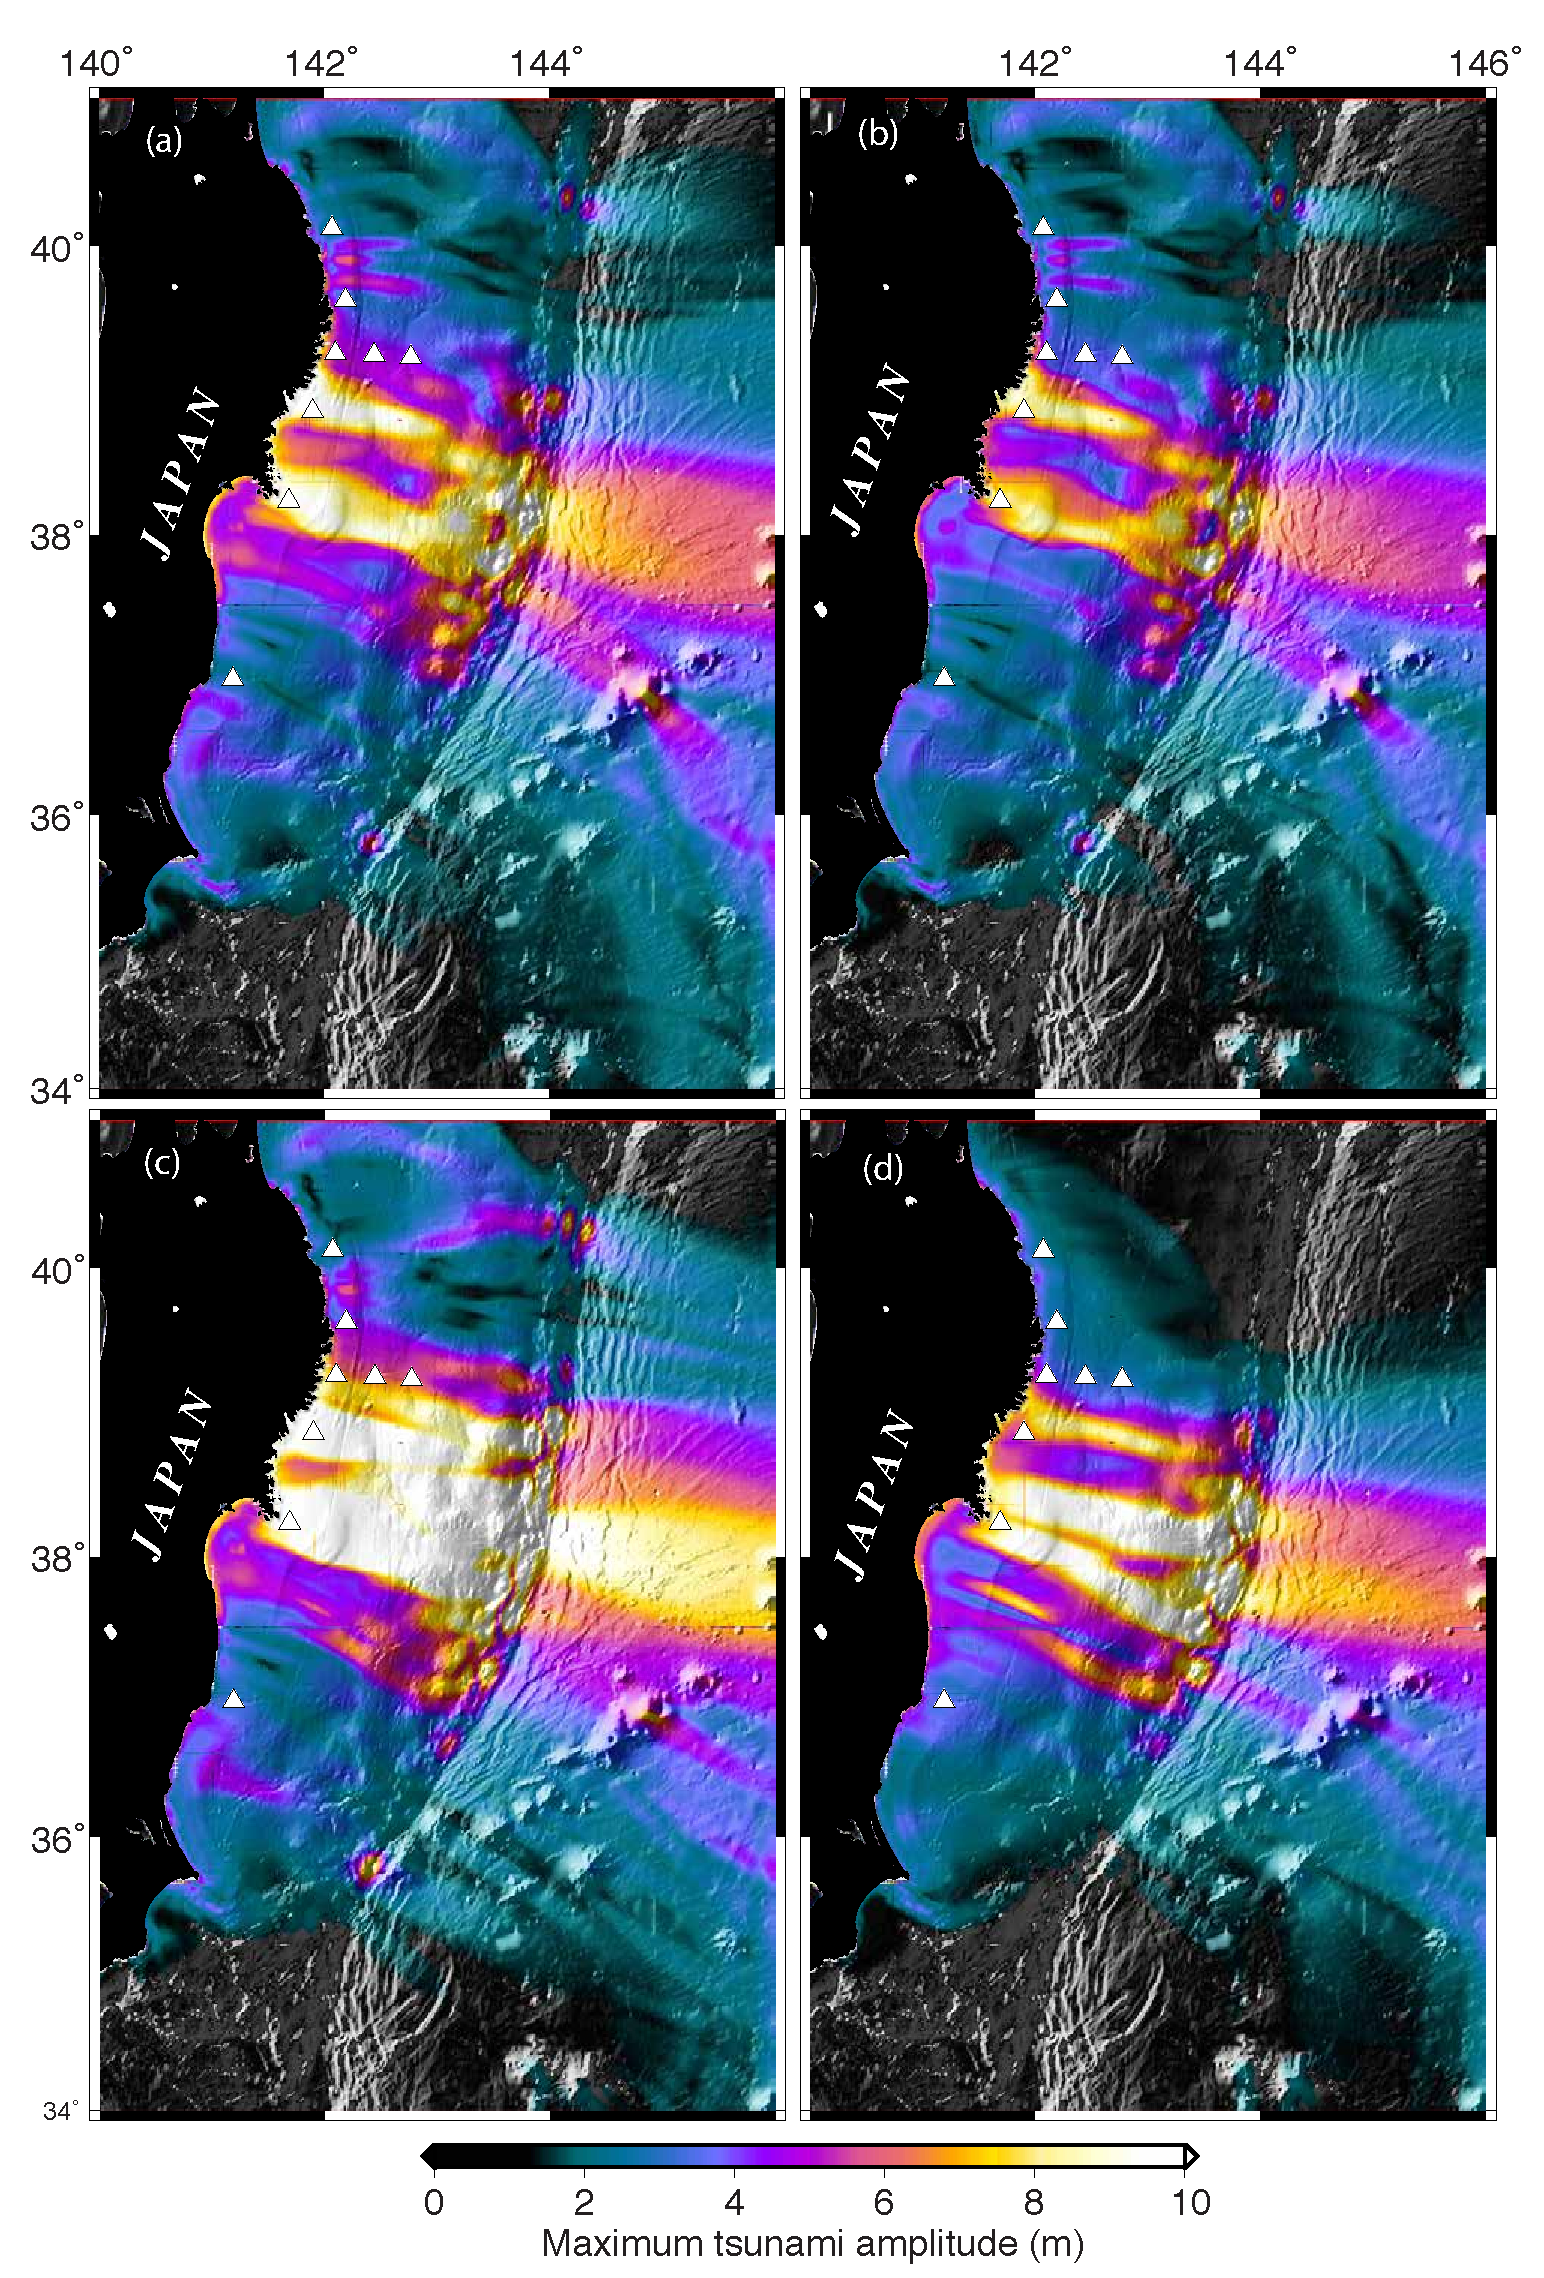
\includegraphics[width=0.78\linewidth]{./figures/ch5/inundation_panels.pdf}
    \caption[Maximum tsunami amplitude with kinematic solution]{Maximum tsunami amplitudes with several source models. (a) is the model from the kinematic  joint inversion of land- and ocean-based data. (b) Is the model from the joint kinematic inversion with the contributions of the horizontal motion of bathymetry removed. (c) Is the model from the joint inversion but applied instantaneously as a static model. (d) Is the model resulting from the land-based only kinematic inversion of Chapter 4}
  \label{fig_maxtsun}
\end{figure}

The result in Figure \ref{fig_maxtsun}c is interesting. This is the maximum tsunami amplitude that results from applying the deformation pattern of the joint solution instantaneously, as we did for the static cases in Section \ref{sec:method}. The expected maximum amplitude is significantly larger. This can be understood by studying Figure \ref{fig_tsunamigenesis} where we plot snapshots of the first 180s of tsunami propagation on a trench-perpendicular profile for both the kinematic and the static initial condition. Even though the total final uplift is the same for both models, for the static initial condition this deformation pattern is applied instantaneously and the resulting initial tsunami peak is as large as the maximum uplift in the model (22m). The tsunami wave then propagates outwards. In the kinematic initial conditions we observe a smoother transition from the rest state to the uplift of the sea surface. Additionally, recall that tsunami propagation speed is $\sqrt{gH}$ where $g$ is the acceleration due to gravity and $H$ the water depth. Water depths of 3000-8000m between the shelf break and the trench yield propagation velocities of 10 to 17 km/min. This means that there is ample time during the approximately 3 minutes of source duration for the tsunami waves to propagate away from their particular source regions and interfere with tsunami waves being generated elsewhere. This also explains why at basin-wide distances considering a kinematic versus a static source has little impact on propagation modeling \citep{fujii2007}, as time progresses the differences between the two become smaller. 

\begin{figure}[!ht] 
  \centering
  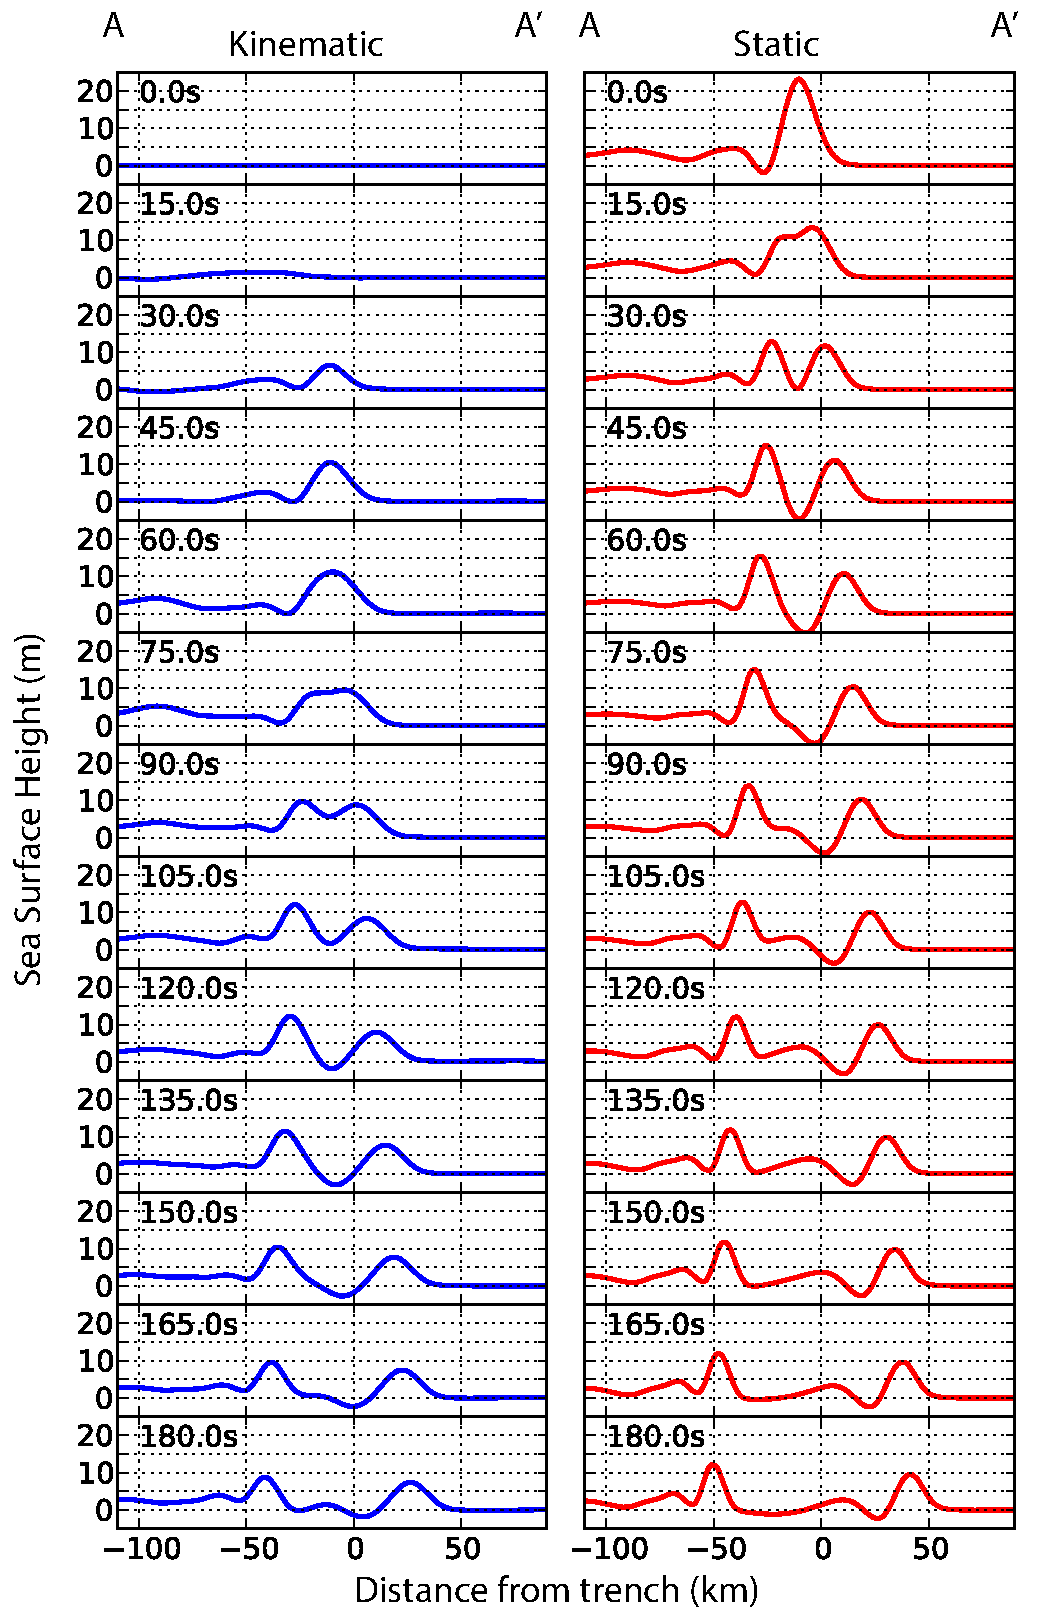
\includegraphics[width=0.59\linewidth]{./figures/ch5/AA.pdf}
    \caption[Trench perpendicular profile of tsunami propagation]{Trench perpendicular profile of tsunami propagation along profile A-A' (Figure \ref{fig_dvt_uplift}). Shown are snapshots of the first 180s of tsunami propagation for (left) the kinematic initia condition and (right) the static initial condition)}
  \label{fig_tsunamigenesis}
\end{figure}

These results do not mean however, that static source models produce larger tsunami amplitudes. When we use static tsunami GFs as in Figure \ref{fig_forecast} we obtain similar maximum expected amplitudes. With static tGFs the inversion process adjusts by placing slip elsewhere  on the slab in order to account for the observed time series at the wave gauges. Rather the importance of this relies in that if a tsunami modeler use a seismically derived kinematic model as an initial condition to study near-field tsunami propagation \citep{macinnes2013} then they will most likely obtain larger amplitudes if applying it as a static model. We find that accounting for the time-dependent deformation of bathymetry is important. Finally, in Figure \ref{fig_maxtsun}d we plot the maximum expected tsunami amplitude using the land-only kinematic inversion as the initial condition. The pattern is similar but in general smaller, this is unsurprising considering the joint model places more slip at the trench than the land-only model. However it does underscore that even if wave gauges are unavailable an earthquake source model derived from regional seismic and geodetic data can provide a much improved estimate of the tsunami intensity. There are still significant improvements to be made, with both the static and kinematic initial conditions we've assumed that the water column responds instantaneously to the vertical motion of the sea floor. Realistically there is a finite time over which the sea-floor deformation is transferred to the sea-surface. This can be modeled as a super-position of acoustic waves \citep{ohmachi2001}, but there are few studies that take this into account and the magnitude of the error incurred from neglecting acoustic waves is unclear. \citet{ohmachi2001} suggests, for example, that when the natural acoustic period of the sea water layer (which depends exclusively one depth) is close to that of the oceanic Rayleigh waves then these can be significant tsunamigenic contributors and amplify the sea surface height. At higher frequencies \citet{kozdon2014} have shown that acoustic waves might reflect important characteristics of the shallow source. Future developments should include this extra source term and quantify its importance.



\section{Acknowledgments}

Sections 5.1-5.4 have been published in \textbf{Melgar, D. and Bock, Y. ``Near-Field Tsunami Models with Rapid Earthquake Source Inversions from Land- and Ocean-Based Observations: The Potential for Forecast and Warning'', \emph{J. Geophys. Res.}, 118(11), 2013}. This research was funded by the NASA Earth and Space Science Fellowship NNX12AN55H, and NASA AIST-11 NNX09AI67G and ROSES NNX12AK24G awards. Brendan Crowell developed and selflessly shared the first version of the coseismic inversion code that is the kernel of the joint inversion code. Discussions with Randy LeVeque and David George were invaluable to our understanding of tsunami science and modeling. We are indebted to Emanuel Garcia, Xiaopeng Tong, Paul Wessel, and David Sandwell for their assistance with manipulation of the topography and bathymetry data sets. Ergin Ulutas provided helpful pointers on dealing with the wave gauge measurements. This work was largely conceived during the 2012 Gene Golub SIAM Summer School on Simulation and Supercomputing in the Geosciences and the 2013 Pan-American Advanced Sciences Institute on The science of predicting and understanding tsunamis, storm surges and tidal phenomena. We are grateful to the organizers, lecturers, and students at both those workshops. We extend our thanks to the Japanese Meteorological Agency for access to accelerometer and tide gauge data; the Geospatial Information Authority for access to GPS data, the Earthquake Research Institute for access to ocean-bottom pressure data, and the Nationwide Ocean Wave information network for GPS buoy data. GeoClaw is available from the developers at http://www.clawpack.org. 




